% Copyright 2025 Fausto Spoto
%
% Licensed under the Apache License, Version 2.0 (the "License");
% you may not use this file except in compliance with the License.
% You may obtain a copy of the License at
%
%    http://www.apache.org/licenses/LICENSE-2.0
%
% Unless required by applicable law or agreed to in writing, software
% distributed under the License is distributed on an "AS IS" BASIS,
% WITHOUT WARRANTIES OR CONDITIONS OF ANY KIND, either express or implied.
% See the License for the specific language governing permissions and
% limitations under the License.

%\RequirePackage{luatex85}
\documentclass[11pt]{beamer}  %% versione proiettore
%%\documentclass[11pt,handout]{beamer} %% versione stampa
\usepackage{lucidiJb-2ed}

\usepackage{animate}
\usepackage{mathtools}
\usepackage{relsize}
\usepackage[normalem]{ulem}
\usepackage[dvipsnames]{xcolor}
\usepackage{amsmath}
\usepackage{amssymb}
\usepackage{amsfonts}
\usepackage{tikz}
%\usetikzlibrary {arrows.meta,graphs,graphdrawing}
%\usegdlibrary{layered}
%\usegdlibrary{trees}
\usetikzlibrary{decorations.pathreplacing}
\usetikzlibrary {arrows.meta}
\usepackage{algorithm,algpseudocode}
\usepackage{listings}

\lstset{
  breakatwhitespace,
  language=MATLAB,
  columns=fullflexible,
  keepspaces,
  breaklines,
  tabsize=3, 
  showstringspaces=false,
  extendedchars=true,
  basicstyle=\fontfamily{pcr}\selectfont\scriptsize,
  keywordstyle=\color{orange},
  upquote=true,
  literate={-}{-}1}

\renewcommand{\algorithmicrequire}{\textbf{Input:}}
\renewcommand{\algorithmicensure}{\textbf{Output:}}

\mode<article>
{
  \usepackage{fullpage}
  \usepackage{hyperref}
}

\mode<presentation>
{
  \setbeamertemplate{background canvas}[vertical shading][bottom=red!10,top=blue!10]
  \usetheme{Course}
  \usefonttheme[onlysmall]{structurebold}
}

\newcommand{\wrt}{\textit{wrt.\ }}
\newcommand{\ie}{, \textit{ie.}, }

\newcommand{\numberofscoops}{{\#\mathit{scoops}}}
\newcommand{\noncesize}{{\mathit{nonce}_{\mathit{size}}}}
\newcommand{\byte}{{\mathit{byte}}}
\newcommand{\nonce}{{\mathit{nonce}}}
\newcommand{\execute}{{\mathit{execute}}}
\newcommand{\bestNonce}{{\mathit{best\_nonce}}}
\newcommand{\nonces}{{\mathit{nonces}}}
\newcommand{\scoops}{{\mathit{scoops}}}
\newcommand{\plot}{{\mathit{plot}}}
\newcommand{\scoop}{{\mathit{scoop}}}
\newcommand{\seed}{{\mathit{seed}}}
\newcommand{\previous}{{\mathit{previous}}}
\newcommand{\deadline}{{\mathit{deadline}}}
\newcommand{\generation}{{\mathit{generation}}}
\newcommand{\size}{{\mathit{size}}}
\newcommand{\scoopnumber}{{\mathit{scoopNumber}}}
\newcommand{\data}{{\mathit{data}}}
\newcommand{\challenge}{{\mathit{challenge}}}
\newcommand{\delay}{{\mathit{delay}}}
\newcommand{\mynext}{{\mathit{next}}}
\newcommand{\nextchallenge}{\challenge_\mynext}
\newcommand{\initialchallenge}{{\mathit{initialChallenge}}}
\newcommand{\finalstateid}{{\mathit{finalStateId}}}
\newcommand{\height}{{\mathit{height}}}
\newcommand{\trunk}{{\mathit{trunk}}}
\renewcommand{\block}{{\mathit{block}}}
\newcommand{\oblivion}{{\mathit{oblivion}}}
\newcommand{\now}{{\mathit{now}}}
\newcommand{\beat}{{\mathit{beat}}}
\newcommand{\weightedbeat}{\mathit{weightedBeat}}
\newcommand{\nextweightedbeat}{\weightedbeat_\mynext}
\newcommand{\power}{{\mathit{power}}}
\newcommand{\hash}{{\mathit{hash}}}
\newcommand{\difficulty}{{\mathit{difficulty}}}
\newcommand{\hashfirstk}{{\mathit{hash\ of\ first\ \kappa\ bytes\ of}}}
\newcommand{\previousblockhash}{{\mathit{previousBlockHash}}}
\newcommand{\waitingtime}{{\mathit{waitingTime}}}
\newcommand{\transactions}{{\mathit{transactions}}}
\newcommand{\nextwaitingtime}{\tau_\mynext}
\newcommand{\nextpower}{\power_\mynext}
\newcommand{\nextacceleration}{\alpha_\mynext}
\newcommand{\nextblock}{\block_\mynext}
\newcommand{\genesis}{{\mathit{genesis}}}
\newcommand{\consensus}{{\mathit{consensus}}}
\newcommand{\nattobe}{{\mathit{nat2be}}}
\newcommand{\betonat}{{\mathit{be2nat}}}
\newcommand{\finalhash}{{h_{\mathit{final}}}}
\newcommand{\chainidentifier}{{\mathit{chainIdentifier}}}
\newcommand{\publickeyofpeer}{{\mathit{publicKeyOfPeer}}}
\newcommand{\publickeyofminer}{{\mathit{publicKeyOfMiner}}}

\newcommand{\Prologs}{{\mathsf{Prologs}}}
\newcommand{\Plots}{{\mathsf{Plots}}}
\newcommand{\Challenges}{{\mathsf{Challenges}}}
\newcommand{\Scoops}{{\mathsf{Scoops}}}
\newcommand{\Nonces}{{\mathsf{Nonces}}}
\newcommand{\Trunks}{{\mathsf{Trunks}}}
\newcommand{\Blocks}{{\mathsf{Blocks}}}
\newcommand{\GenesisBlocks}{{\mathsf{GenesisBlocks}}}
\newcommand{\NonGenesisBlocks}{{\mathsf{NonGenesisBlocks}}}
\newcommand{\Deadlines}{{\mathsf{Deadlines}}}

\newcommand{\computer}{
\includegraphics[width=1.3cm]{pictures/computer}}
\newcommand{\leftArrow}{
\includegraphics[width=0.6cm]{pictures/left_arrow}}
\newcommand{\signature}{
\includegraphics[width=0.3cm]{pictures/signature}}
\newcommand{\leftplug}{
\includegraphics[width=0.7cm]{pictures/plug_left}}
\newcommand{\rightplug}{
\includegraphics[width=0.7cm]{pictures/plug_right}}
\newcommand{\ssd}{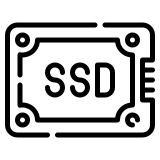
\includegraphics[width=0.8cm]{pictures/ssd}}

\colorlet{alicecolor}{green!90!black}
\colorlet{bobcolor}{red!90!black}
\colorlet{faustocolor}{yellow!90!black}
\colorlet{lightred}{red!50!white}
\colorlet{verylightgray}{gray!25!white}
      
\subtitle{InterReg workshop, Saint-Denis, R\'eunion, 5/11/2025}
\title{Blockchain, Ecological Cryptomining, Mokamint and Hotmoka}
\institute{Universit\`a di Verona, Italy}
\date{5/11/2025}

\setbeamercovered{invisible}

\def\codesize{\smaller}
\def\<#1>{\codeid{#1}}
\newcommand{\codeid}[1]{\ifmmode{\mbox{\codesize\ttfamily{#1}}}\else{\codesize\ttfamily #1}\fi}

\AtBeginSection[]{
  \begin{frame}
  \vfill
  \centering
  \begin{beamercolorbox}[sep=8pt,center,shadow=true,rounded=true]{title}
    \usebeamerfont{title}\insertsectionhead\par%
  \end{beamercolorbox}
  \vfill
  \end{frame}
}

\begin{document}

\begin{frame}
  \titlepage
\end{frame}

\begin{frame}{About myself}
  \begin{itemize}
  \item Associate Professor, Department of Computer Science, University of Verona, Italy
  \item software engineering and verification (1995-today)
  \item smart contracts, consensus, blockchain programming (2018-today)
  \end{itemize}

  \medskip

  \begin{center}
    
\includegraphics[width=3cm]{pictures/verona_map}
  \end{center}

\end{frame}

\begin{frame}
  \frametitle{Outline}
  \begin{center}
    Morning
  \end{center}
  \tableofcontents[part=1]
  \bigskip
  \begin{center}
    Afternoon
  \end{center}
  \tableofcontents[part=2]
\end{frame}

\part{1}

\section{Introduction}
  
\begin{frame}\frametitle{The mainstream view of blockchain}

  \begin{center}
    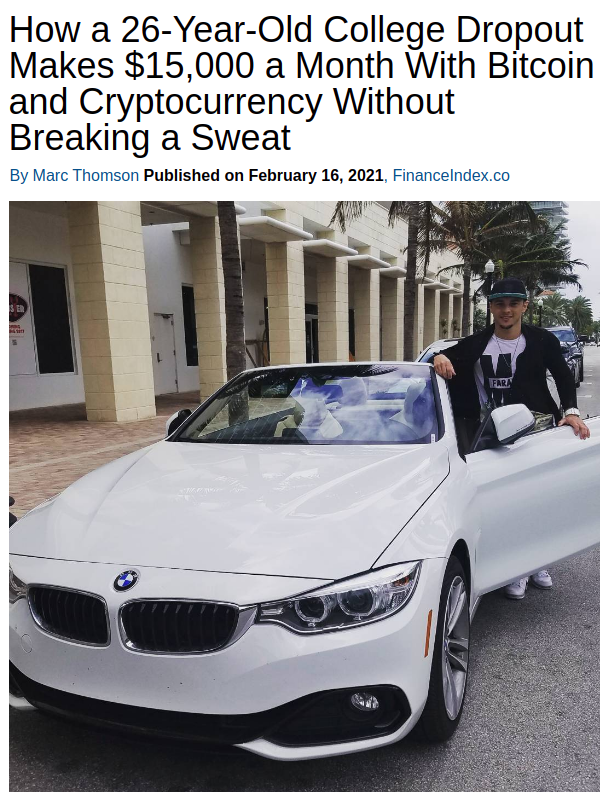
\includegraphics[scale=0.209,clip=false]{pictures/dropout.png}
    \hspace*{2ex}
    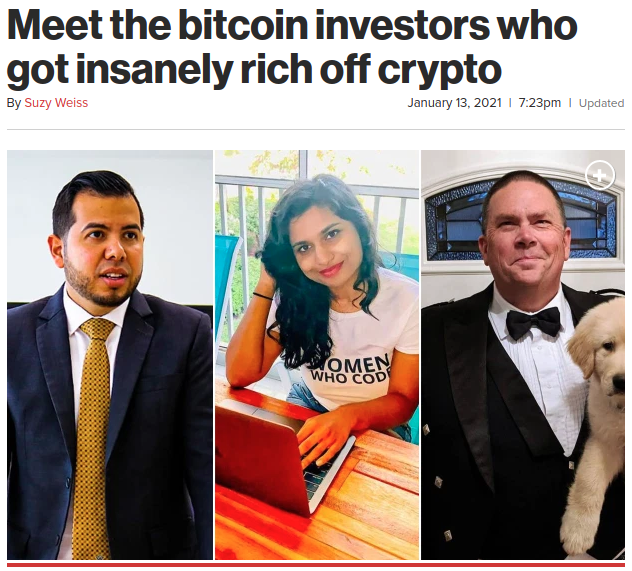
\includegraphics[scale=0.29,clip=false]{pictures/insane.png}
  \end{center}

\end{frame}

\begin{frame}\frametitle{Who issues and moves the money?}

  \begin{center}
    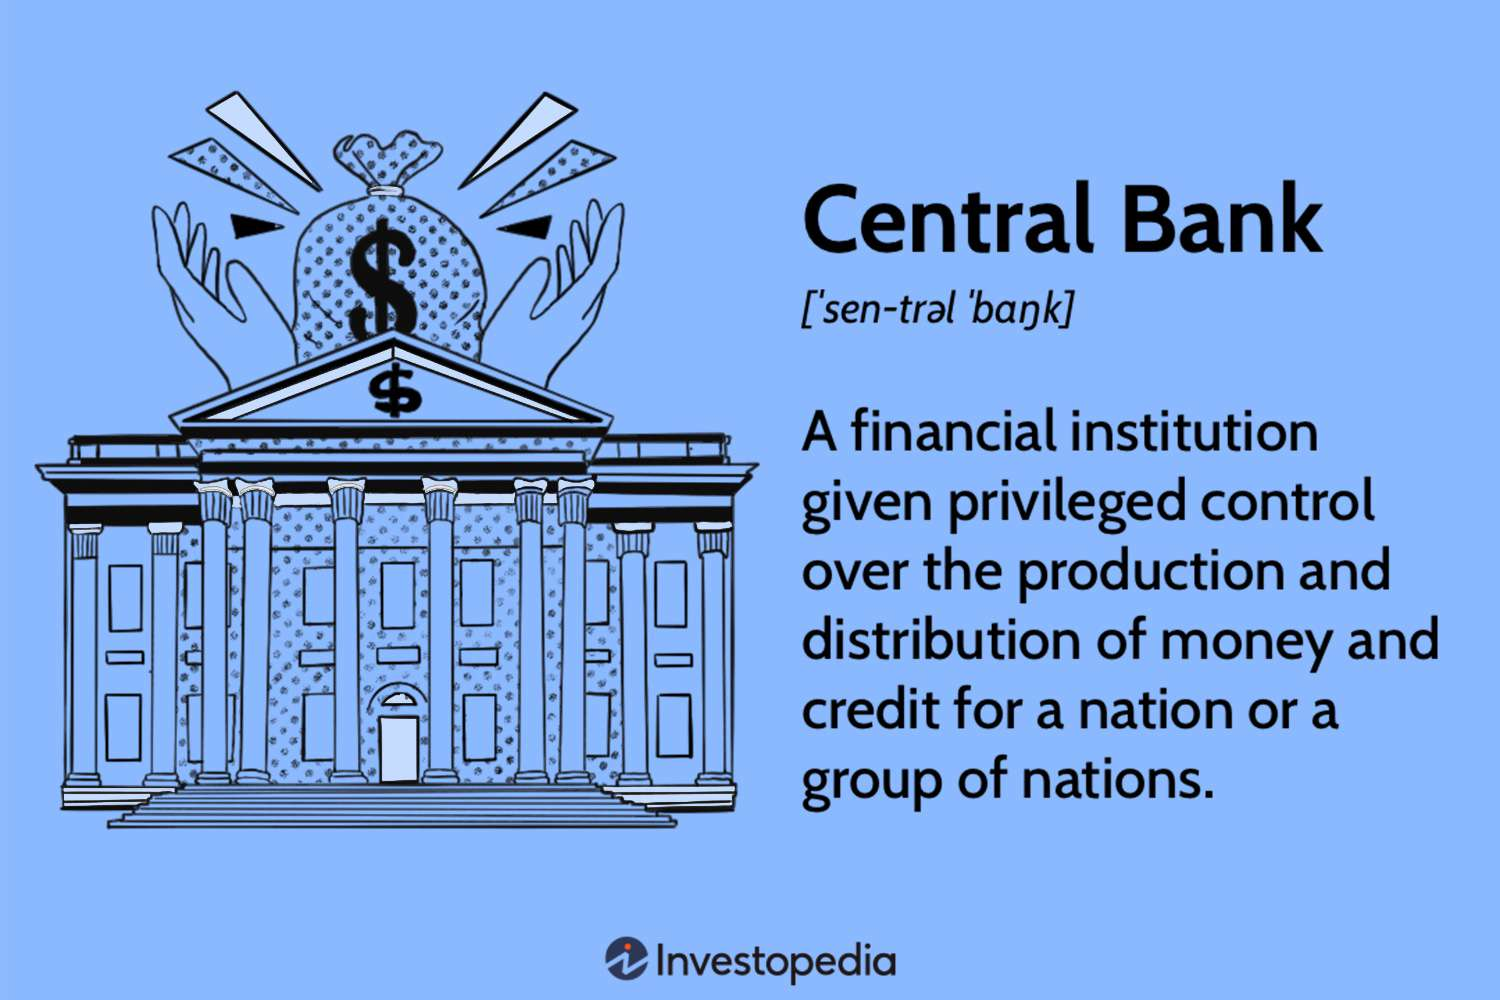
\includegraphics[scale=0.22,clip=false]{pictures/central-bank.jpg}
  \end{center}

\end{frame}

\begin{frame}{Trust is rare in this world}

  \begin{itemize}
  \item we trust our central bank because we must
  \item we trust our supermarket points because they have little and limited value
  \item we trust PayPal because we keep and exchange little money on it
  \item we trust credit card issuers up to a few thousand dollars
    because they \emph{should not} fail
    and \emph{should not} cheat (too big to fail, to big to cheat)
  \end{itemize}

\end{frame}

\begin{frame}\frametitle{Can trust arise in a trusteless world?}

  \begin{greenbox}{We want a money handling system that}
    \begin{itemize}
    \item has no central, special issuer
    \item consists of many computers, all created equal
    \item if some computers fail, the network survives
    \item each computer contains all data, it does not need the others
    \item if a computer holds corrupted data, we can immediately see it
    \item the system is very unlikely to change the history of money transfers
      (no double spending)
    \end{itemize}
  \end{greenbox}

  \begin{center}
    
\includegraphics[scale=0.3,clip=false]{pictures/unicorn.jpg}
  \end{center}

\end{frame}

\begin{frame}\frametitle{Distributed networks}

  \begin{center}
    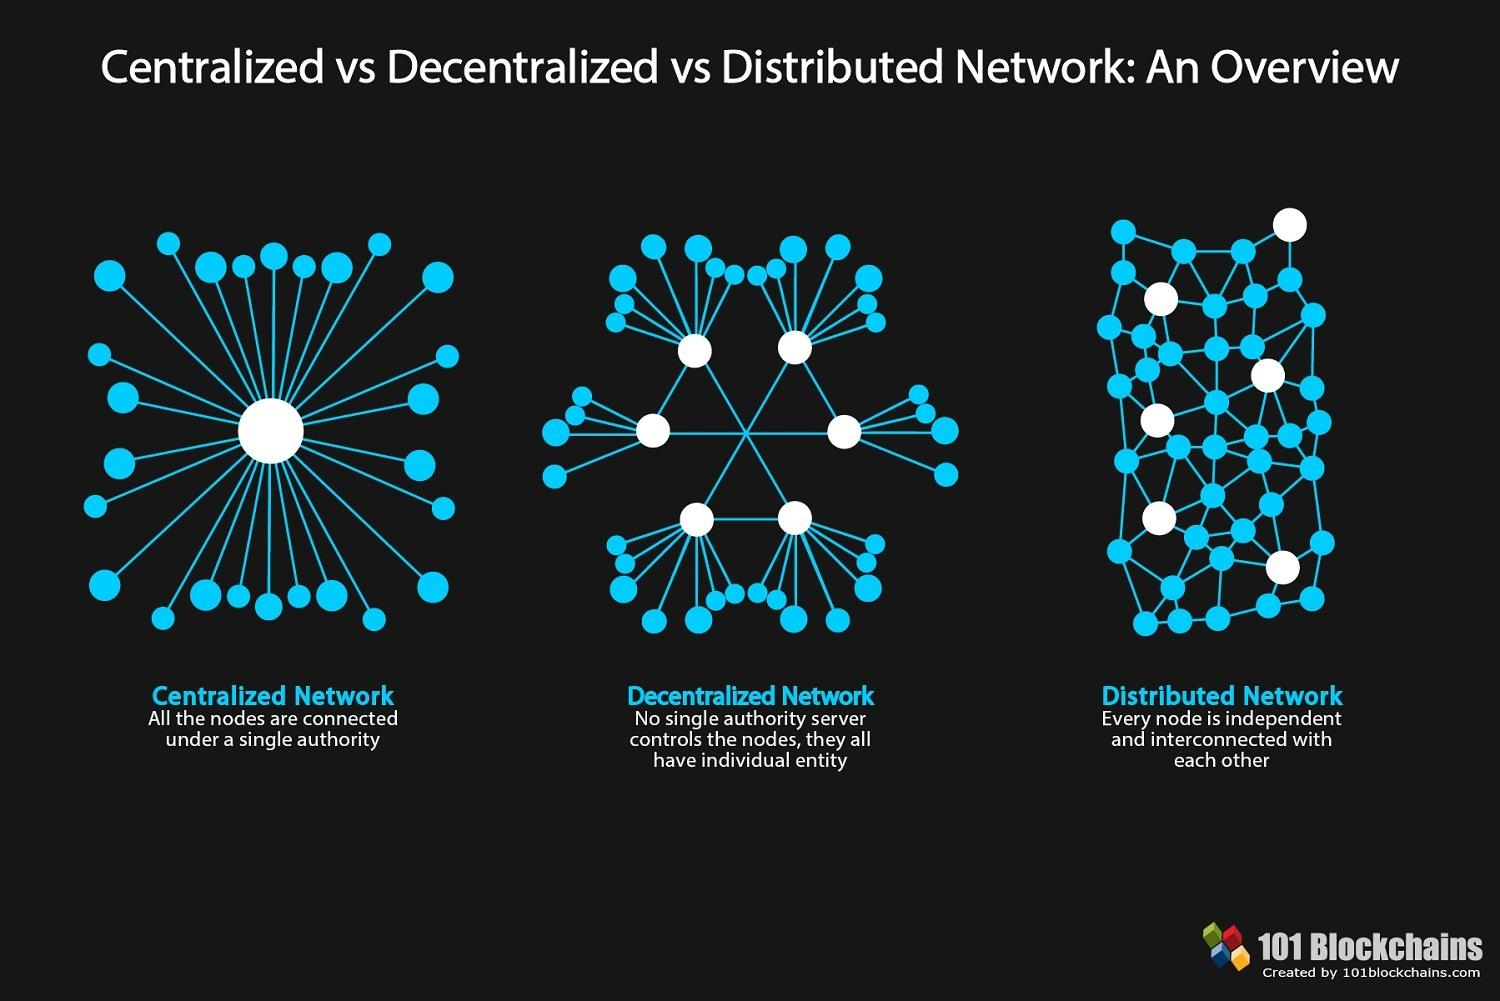
\includegraphics[scale=0.22,clip=false]{pictures/distributed.jpg}
  \end{center}

\end{frame}

\begin{frame}\frametitle{Git: A distributed network}

  \begin{center}
    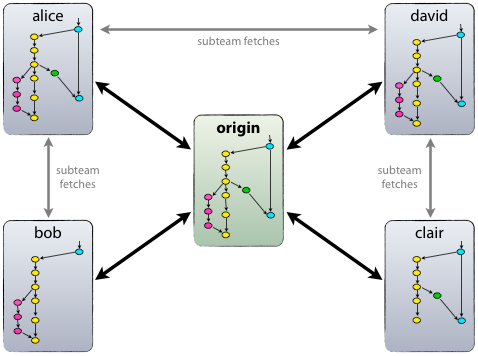
\includegraphics[scale=0.26,clip=false]{pictures/git_distributed.png}
  \end{center}

  \begin{greenbox}{An approximation of what we want}
    \begin{itemize}
    \item no central, special computer
    \item all computers are equal
    \item if some computers fail, the repository survives
    \item each computer contains all data, it does not need the others
    \item if a computer holds corrupted data, we see an inconsistent hash
    \item {\color{red}the system allows diverging evolutions (double spending)}
    \end{itemize}
  \end{greenbox}
  
\end{frame}

\begin{frame}\frametitle{History}

  \begin{itemize}
  \item[1988] Proof of work (Dwork \& Naor)
  \item[1991] Cryptographically secure chains of blocks (Haber \& Stornetta)
  \item[199x] Smart contracts (Szabo)
  \item[2008] Bitcoin (Nakamoto)
  \item[2012] Proof of stake (Peercoin)
  \item[2013] Ethereum (Buterin \& Wood)
  \item[2014] Proof of space (Burstcoin then Signum)
  \item[2014] Tendermint generic proof of stake engine (Kwon)
  \item[2022] Ethereum 2.0 adopts the proof of stake
  \item[2022] Bitcoin remains the only blockchain still using the proof of work 
  \end{itemize}
  
\end{frame}

\begin{frame}\frametitle{Bitcoin capitalization (2025)}

  \begin{center}
    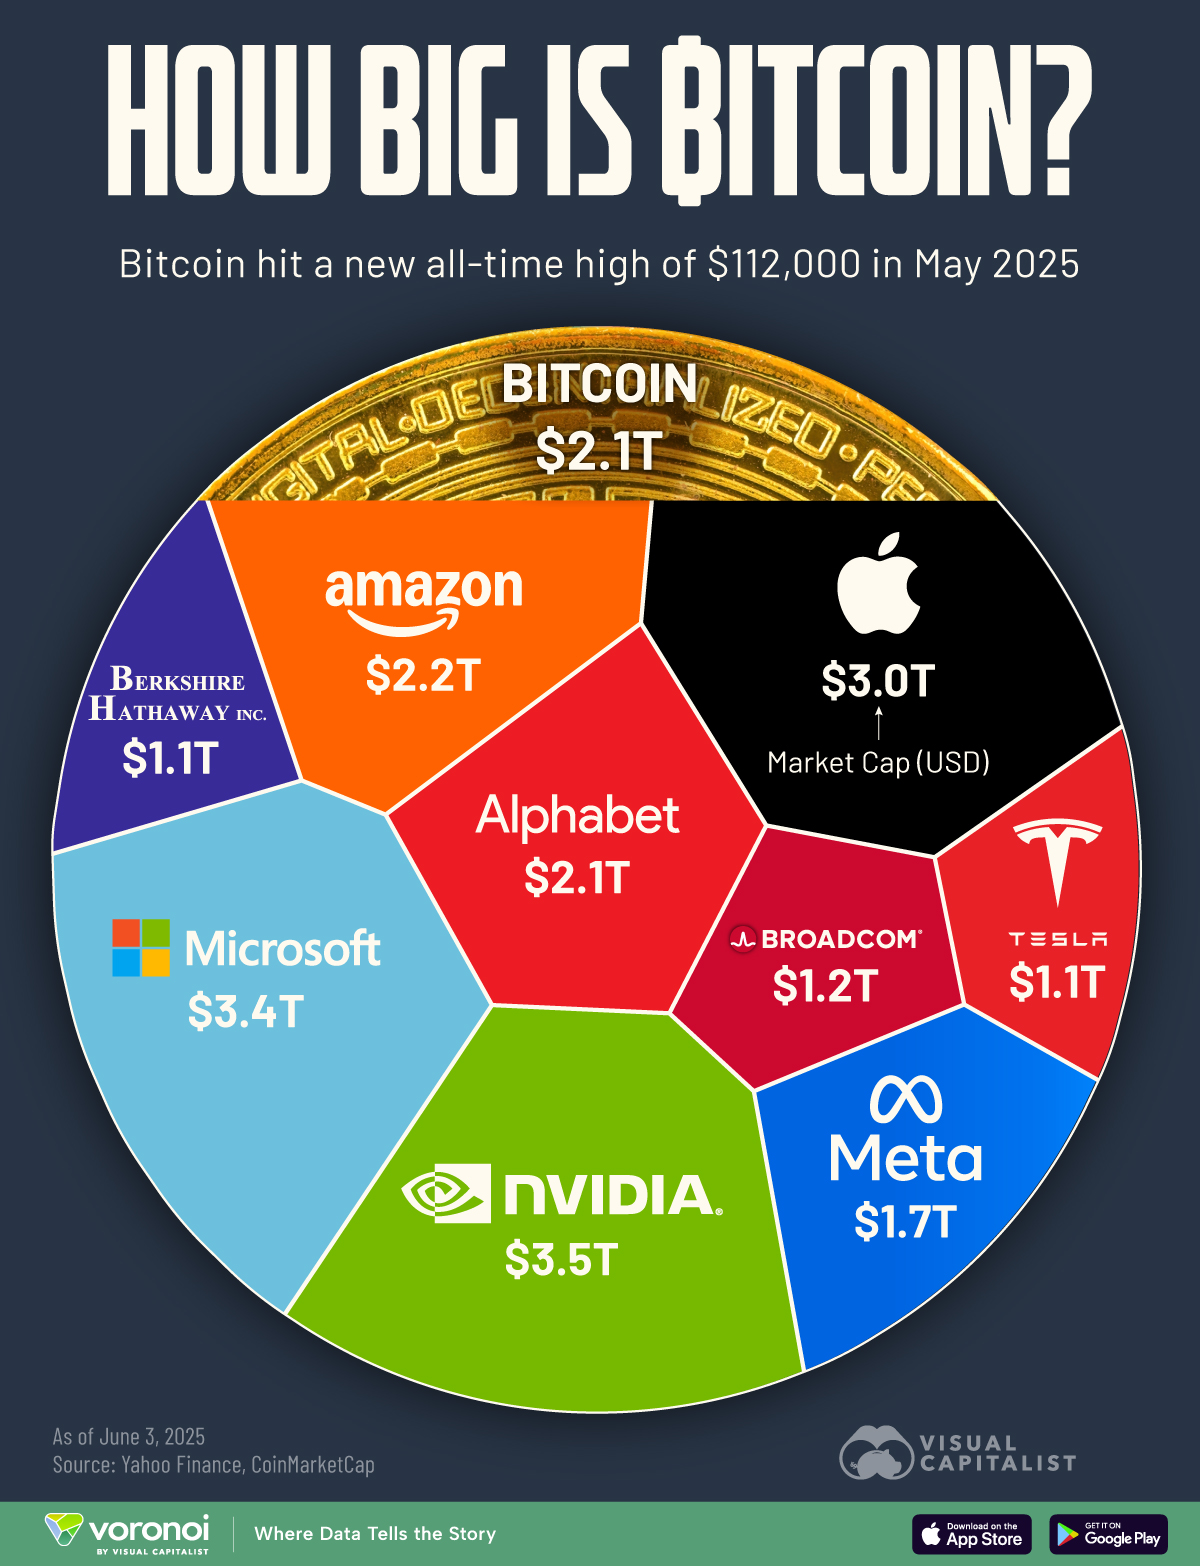
\includegraphics[scale=0.13,clip=false]{pictures/bitcoin-capitalization-2025.jpg}
  \end{center}

  \begin{center}
    source: Yahoo Finance, CoinMarketCap
  \end{center}

\end{frame}

\begin{frame}\frametitle{Ethereum: Bitcoin + Turing}

  Ethereum generalized Bitcoin's money transactions (decidable, terminating) to
  Turing-complete code-driven transactions (undecidable, possibly non-terminating)
  
  \begin{center}
    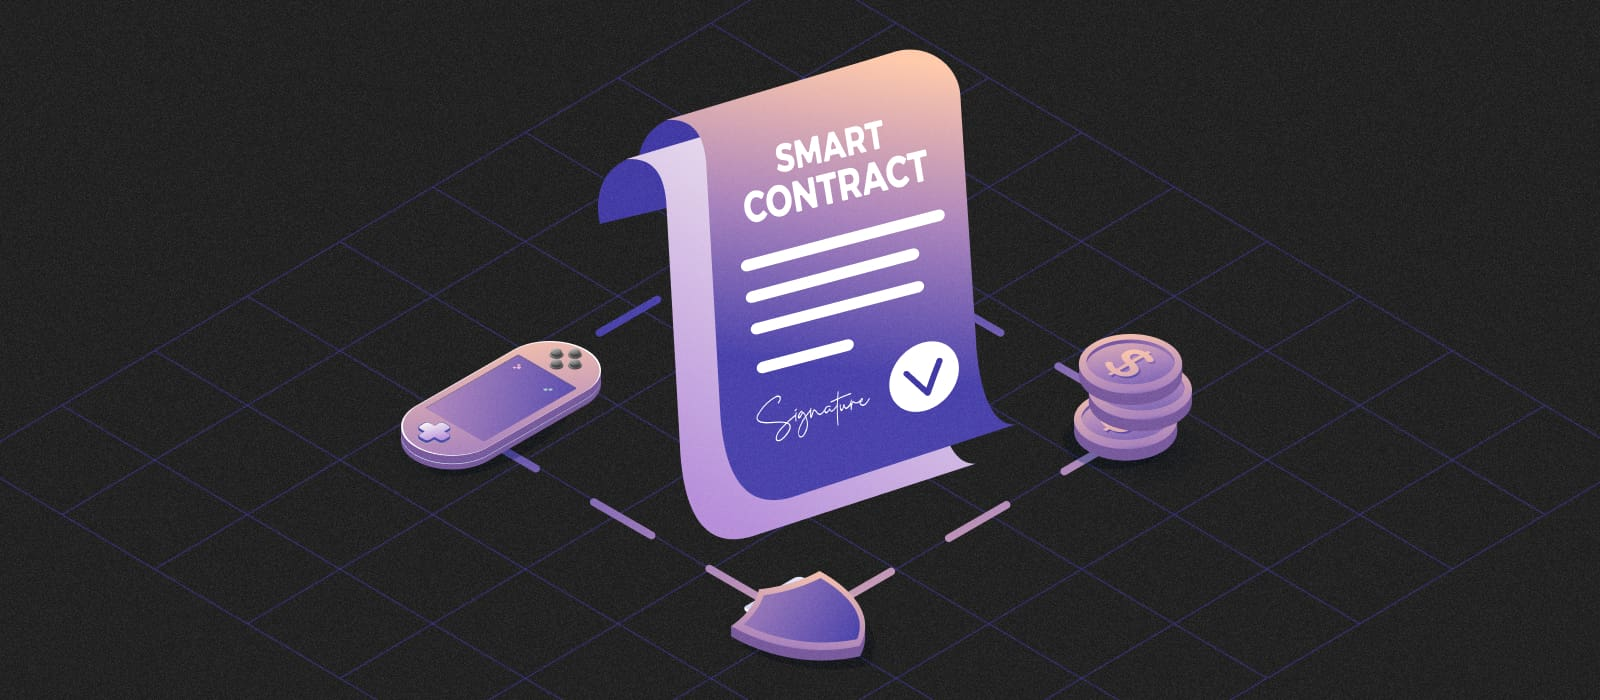
\includegraphics[scale=0.18,clip=false]{pictures/smart-contract.jpg}
  \end{center}

\end{frame}

\begin{frame}\frametitle{Beyond the hype}

  \begin{center}
    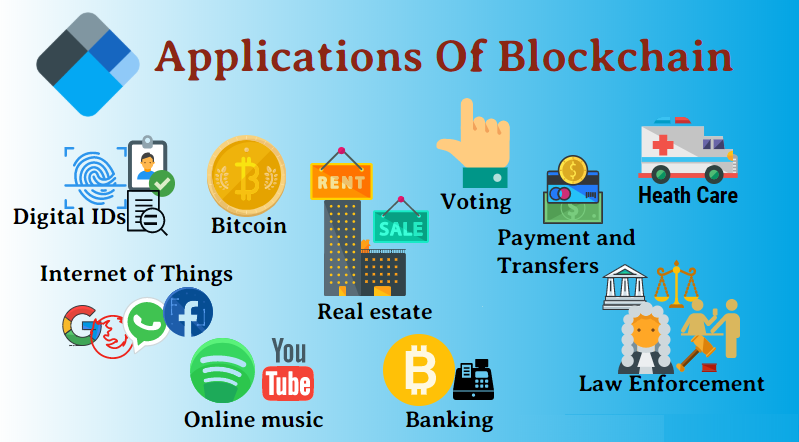
\includegraphics[scale=0.4,clip=false]{pictures/blockchain-applications.png}
  \end{center}

\end{frame}

\begin{frame}\frametitle{The hype cycle}

  \begin{center}
    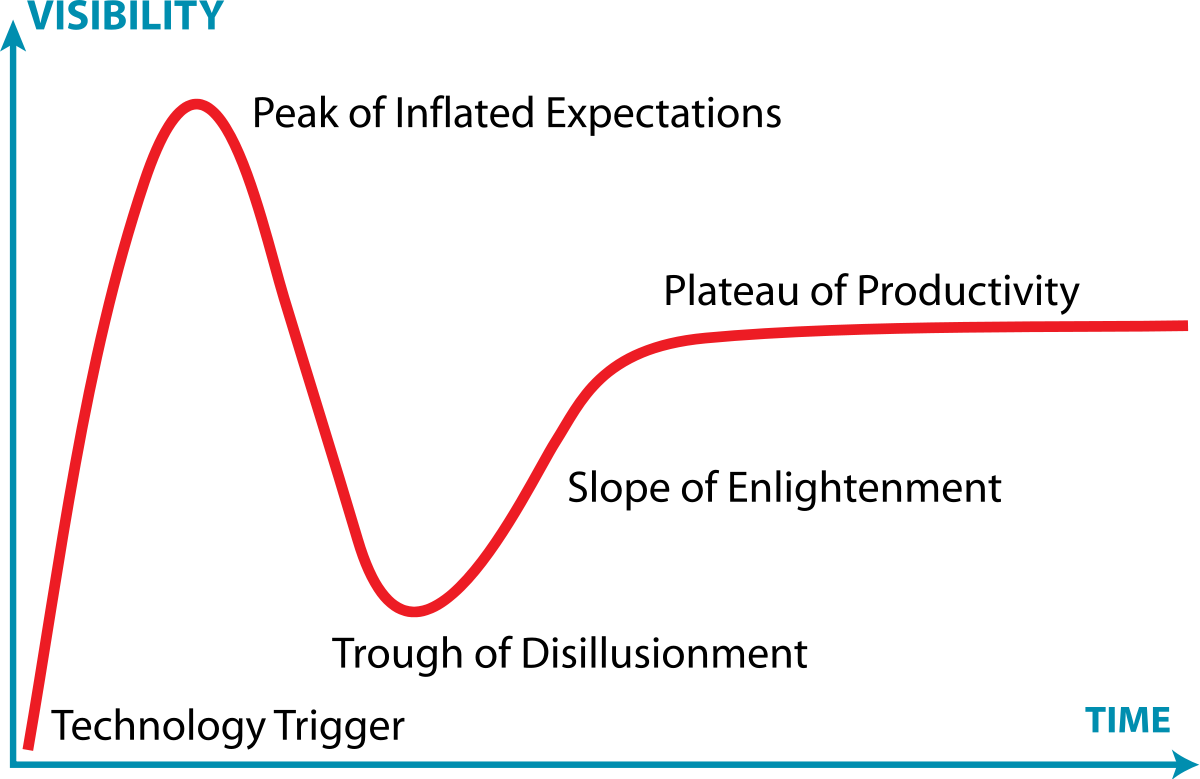
\includegraphics[width=\textwidth,clip=false]{pictures/hype-cycle.png}
  \end{center}

\end{frame}

\section{Bitcoin and its proof of work}

\begin{frame}\frametitle{A secure chain of blocks}

  \begin{center}
    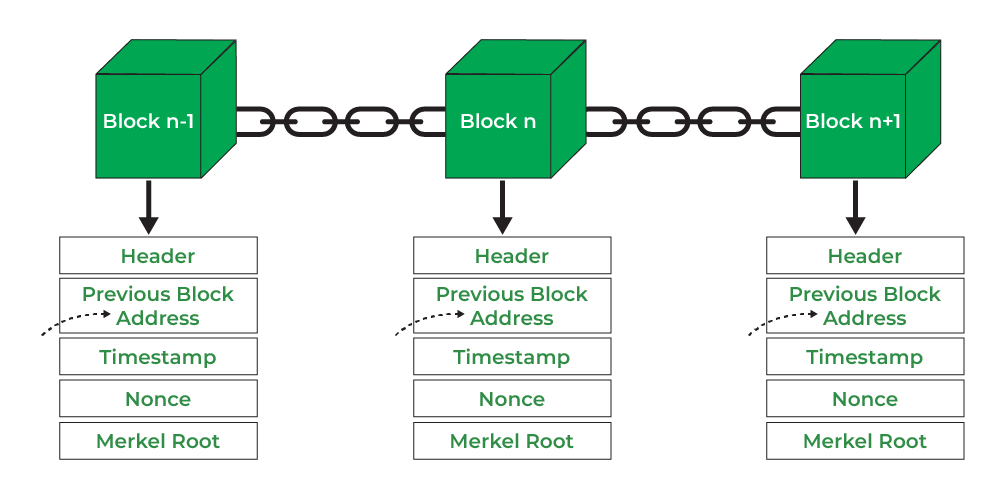
\includegraphics[scale=0.26,clip=false]{pictures/blocks.png}
  \end{center}

  Hashes are used as machine-independent backwards pointers.
  If one modifies data in block $n$, then its hash changes and consequently
  blocks $n+1$, $n+2$, \ldots
  must be modified as well.

  \medskip

  \begin{redbox}{}
    But recomputation is possible in a few seconds for a modern computer
  \end{redbox}
  
\end{frame}

\begin{frame}\frametitle{Proof of work}

  \begin{redbox}{}
    Cynthia Dwork and Noni Naor (1992). \emph{Pricing via Processing, Or, Combatting Junk Mail}. Advances in Cryptology (CRYPTO’92): Lecture Notes in Computer Science No. 740. Springer: 139–147.
  \end{redbox}

  \bigskip

  \begin{tabular}{ccc}
    $\begin{array}{c}
      \text{text of email}\\
      \text{+ recipient address}\\
      \text{+ date of the email}\\
      \text{+ numerical nonce}
    \end{array}$ &
    $\begin{array}{c}
      \text{hashing}\\
      \Rightarrow
    \end{array}$ &
    $\mathtt{\underbrace{\color{blue}{\mathtt{fffffff}}}_{\begin{array}{c}7\text{ bits}\\(difficulty)\end{array}}\hspace*{-2.1ex}43f5e6bc00d\ldots5974eda}$
  \end{tabular}

  \bigskip

  The email client will accept the email only if its hash starts with at least seven \texttt{f}'s.

  \medskip

  The sender needs to try and retry hashing for different nonces, until he finds a good hash that will be accepted.

  \medskip

  This takes time and consumes energy: it makes spam expensive.

\end{frame}

\begin{frame}\frametitle{Bitcoin = Secure chain of blocks + Proof of work}

  \begin{center}
    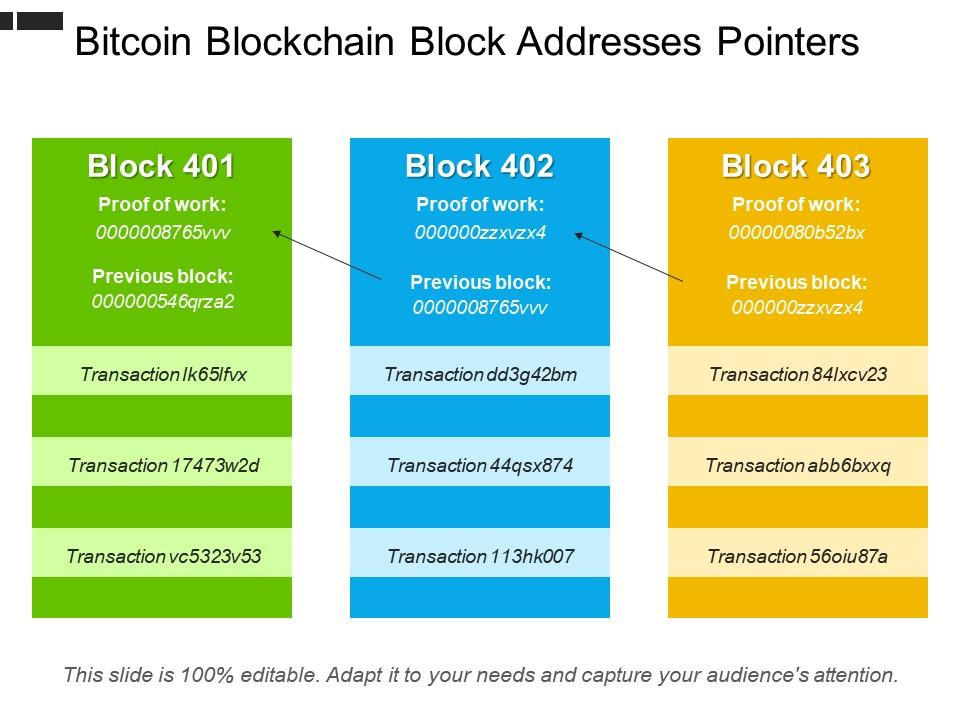
\includegraphics[scale=0.28,clip=false]{pictures/blocks-pow.jpg}
  \end{center}

  \smallskip

  If one modifies data in block $n$, then its hash changes and consequently
  blocks $n+1$, $n+2$, \ldots
  must be modified as well, but this requires to recompute the proof of work
  (a correct nonce for each recomputed block).

  \smallskip

  \begin{redbox}{}
    Recomputation could take centuries even on a very fast computer
  \end{redbox}
\end{frame}

\begin{frame}\frametitle{Proof of work is a worldwide hashing competition}

  People around the world started installing Bitcoin miners, in order to:
  \begin{enumerate}
  \item hash new blocks as quick as possible (brute force)
  \item hope to get the best hash for each new block
  \item earn the per-block prize if they succeed
  \end{enumerate}
\end{frame}

\begin{frame}\frametitle{Bitcoin's energy consumption over the years}

  \begin{center}
    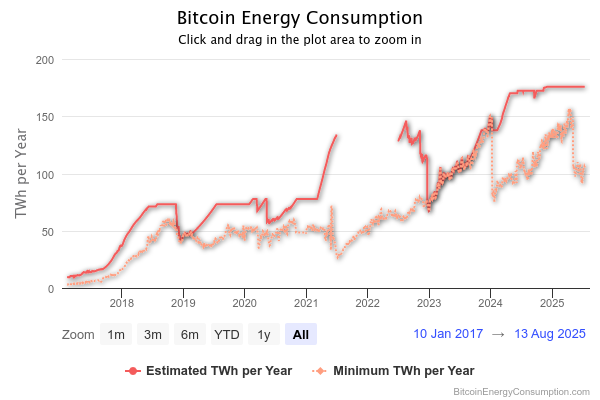
\includegraphics[width=0.9\textwidth,clip=false]{pictures/bitcoin-energy-consumption}
  \end{center}

  \begin{center}
    {\tiny (source: \url{https://digiconomist.net/bitcoin-energy-consumption})}
  \end{center}

\end{frame}

\begin{frame}\frametitle{Annualized Bitcoin's total footprint}

  \begin{center}
    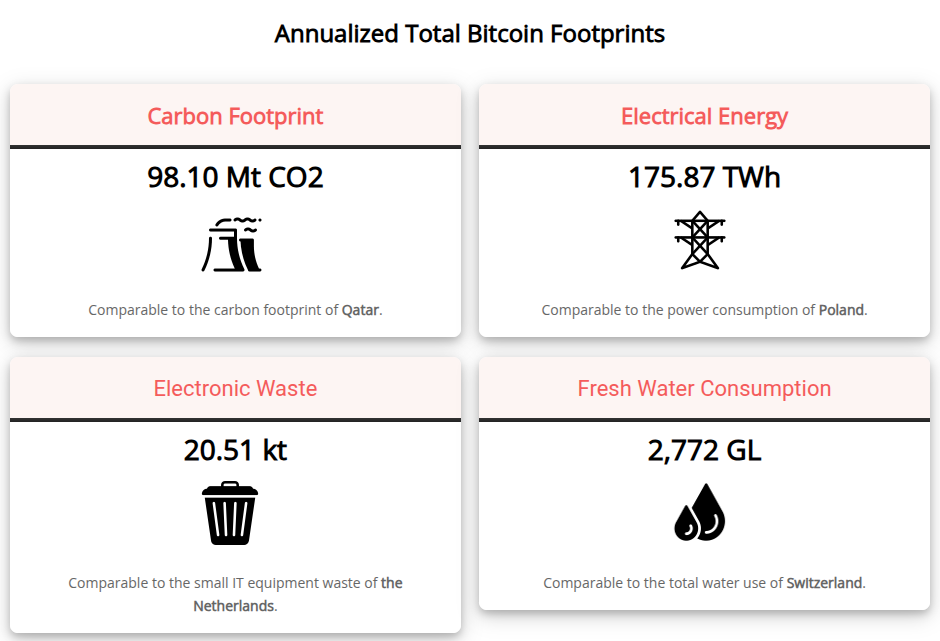
\includegraphics[width=0.85\textwidth,clip=false]{pictures/footprint-annual}
  \end{center}

  \begin{center}
    {\tiny (source: \url{https://digiconomist.net/bitcoin-energy-consumption})}
  \end{center}

\end{frame}

\begin{frame}\frametitle{Bitcoin's footprint for a single transaction}

  \begin{center}
    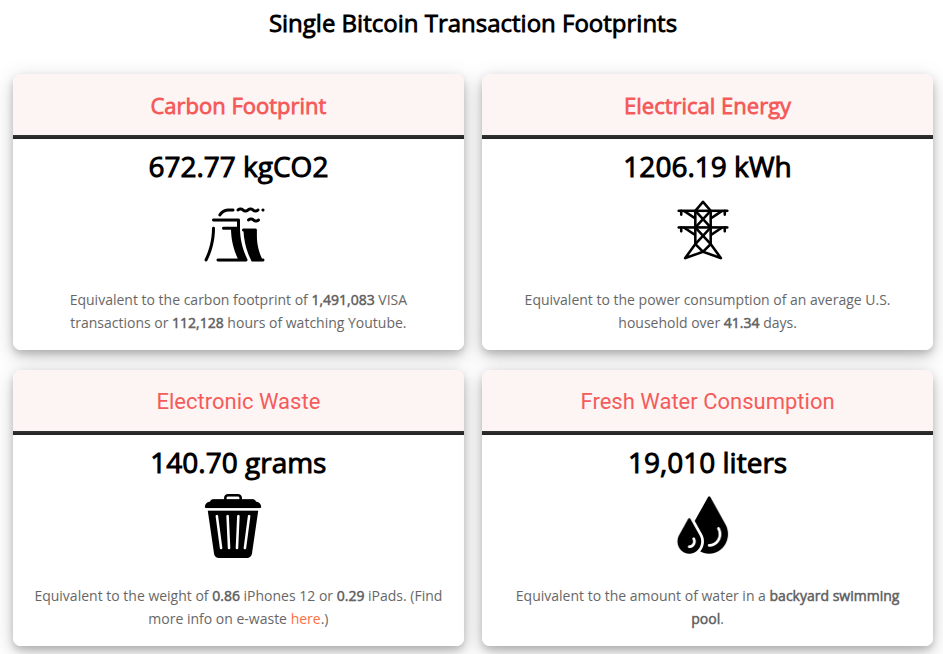
\includegraphics[width=0.85\textwidth,clip=false]{pictures/footprint-single}
  \end{center}

  \begin{center}
    {\tiny (source: \url{https://digiconomist.net/bitcoin-energy-consumption})}
  \end{center}

\end{frame}

\section{IT and ecology: we have a problem}

\begin{frame}{The IT green dream (1990-2010)}

  \begin{center}
    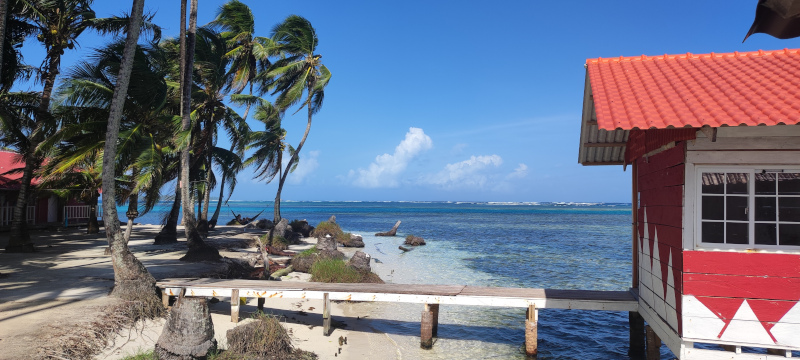
\includegraphics[width=0.7\textwidth]{pictures/green_dream}
  \end{center}

  \begin{center}
    Digital nomads work online from the beach. Calls instead of meetings. No pollution. No war. Peace and love.
  \end{center}

  \begin{center}
    Who needs to think when artificial intelligence things for us?
  \end{center}

  \begin{center}
    Who needs banknotes when we have Bitcoin?
  \end{center}

  \begin{center}
    Who starts a war when we are so social?
  \end{center}

  \begin{center}
    Who needs to drive when cars drive?
  \end{center}

\end{frame}

\begin{frame}{The IT reality (after 2010)}

  \begin{center}
    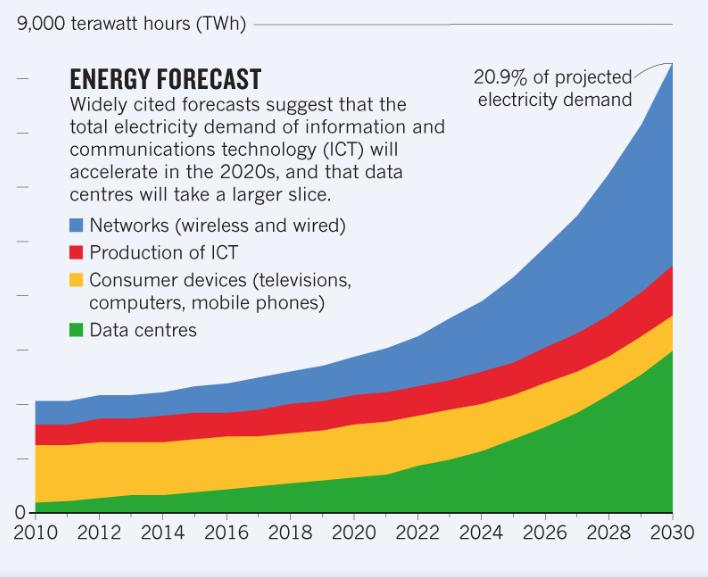
\includegraphics[width=0.7\textwidth]{pictures/forecast}
  \end{center}

  \begin{center}
    {\tiny (source: \url{https://www.capgemini.com/insights/expert-perspectives/the-more-sustainable-data-center/})}
  \end{center}
    
\end{frame}

\begin{frame}{The IT reality (after 2010)}

  \begin{center}
    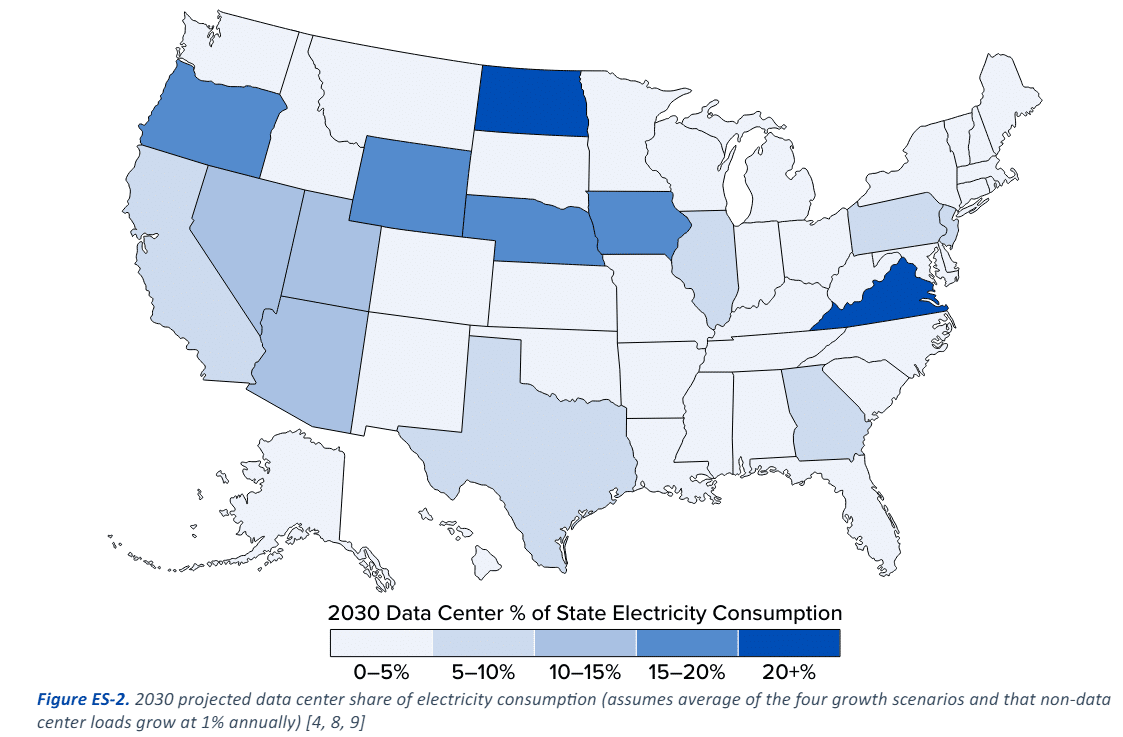
\includegraphics[width=0.7\textwidth]{pictures/data-centers-electricity-use}
  \end{center}

  \begin{center}
    Exercise: find Amazon Web Services in the map.
  \end{center}

  \begin{center}
    {\tiny (source: \url{https://carboncredits.com/us-data-centers-power-requirement-will-double-by-2030/})}
  \end{center}

\end{frame}

\begin{frame}{Not just electricity}

  \begin{center}
    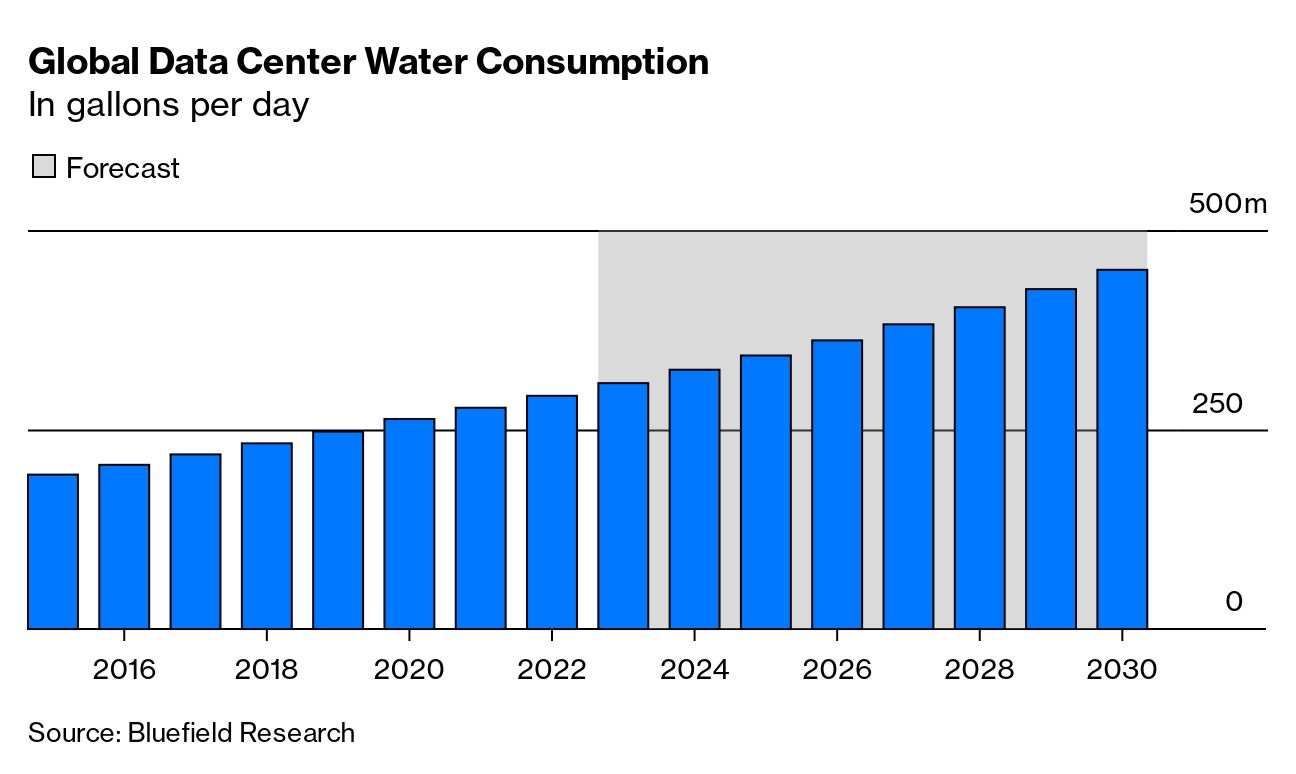
\includegraphics[width=0.8\textwidth]{pictures/water-consumption}
  \end{center}

  \begin{center}
    Data centers need (lot of) water for cooling.
  \end{center}

  \begin{center}
    {\tiny (source: \url{https://siliconangle.com/2024/08/19/environmentalists-sound-alarm-virginias-data-centers-water-consumption-skyrockets/})}
  \end{center}

\end{frame}

\begin{frame}{The disaster is already here}

  \begin{center}
    The Colorado valley is not colored anymore!
  \end{center}

  \begin{center}
    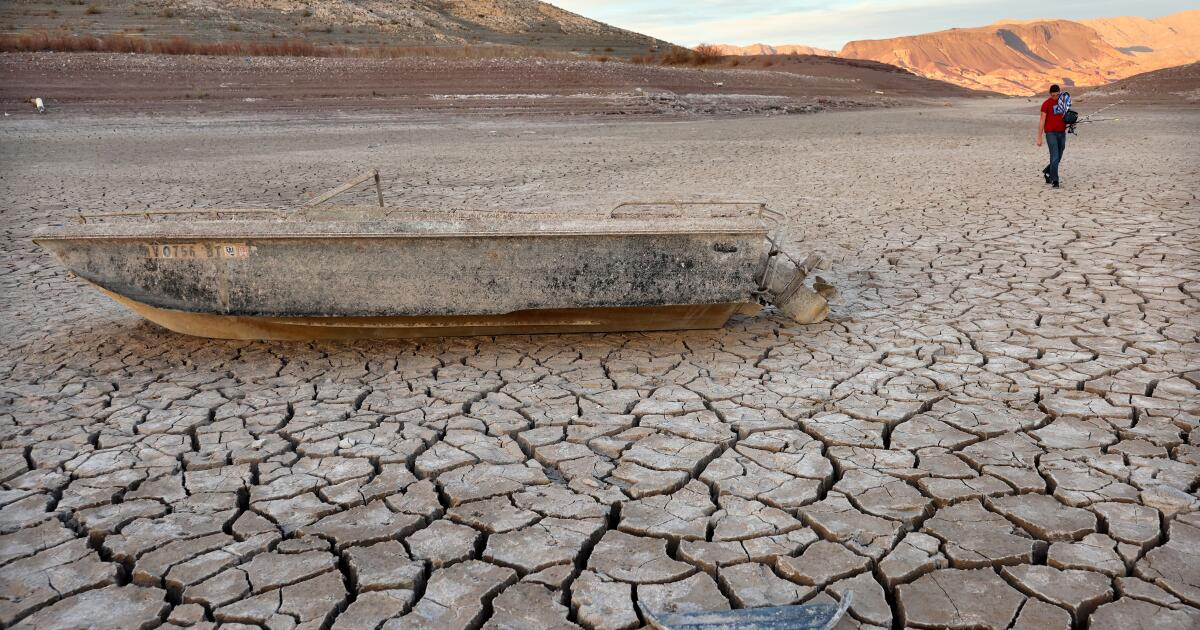
\includegraphics[width=0.75\textwidth]{pictures/colorado}
  \end{center}

\end{frame}

\begin{frame}{Not just electricity}

  \begin{center}
    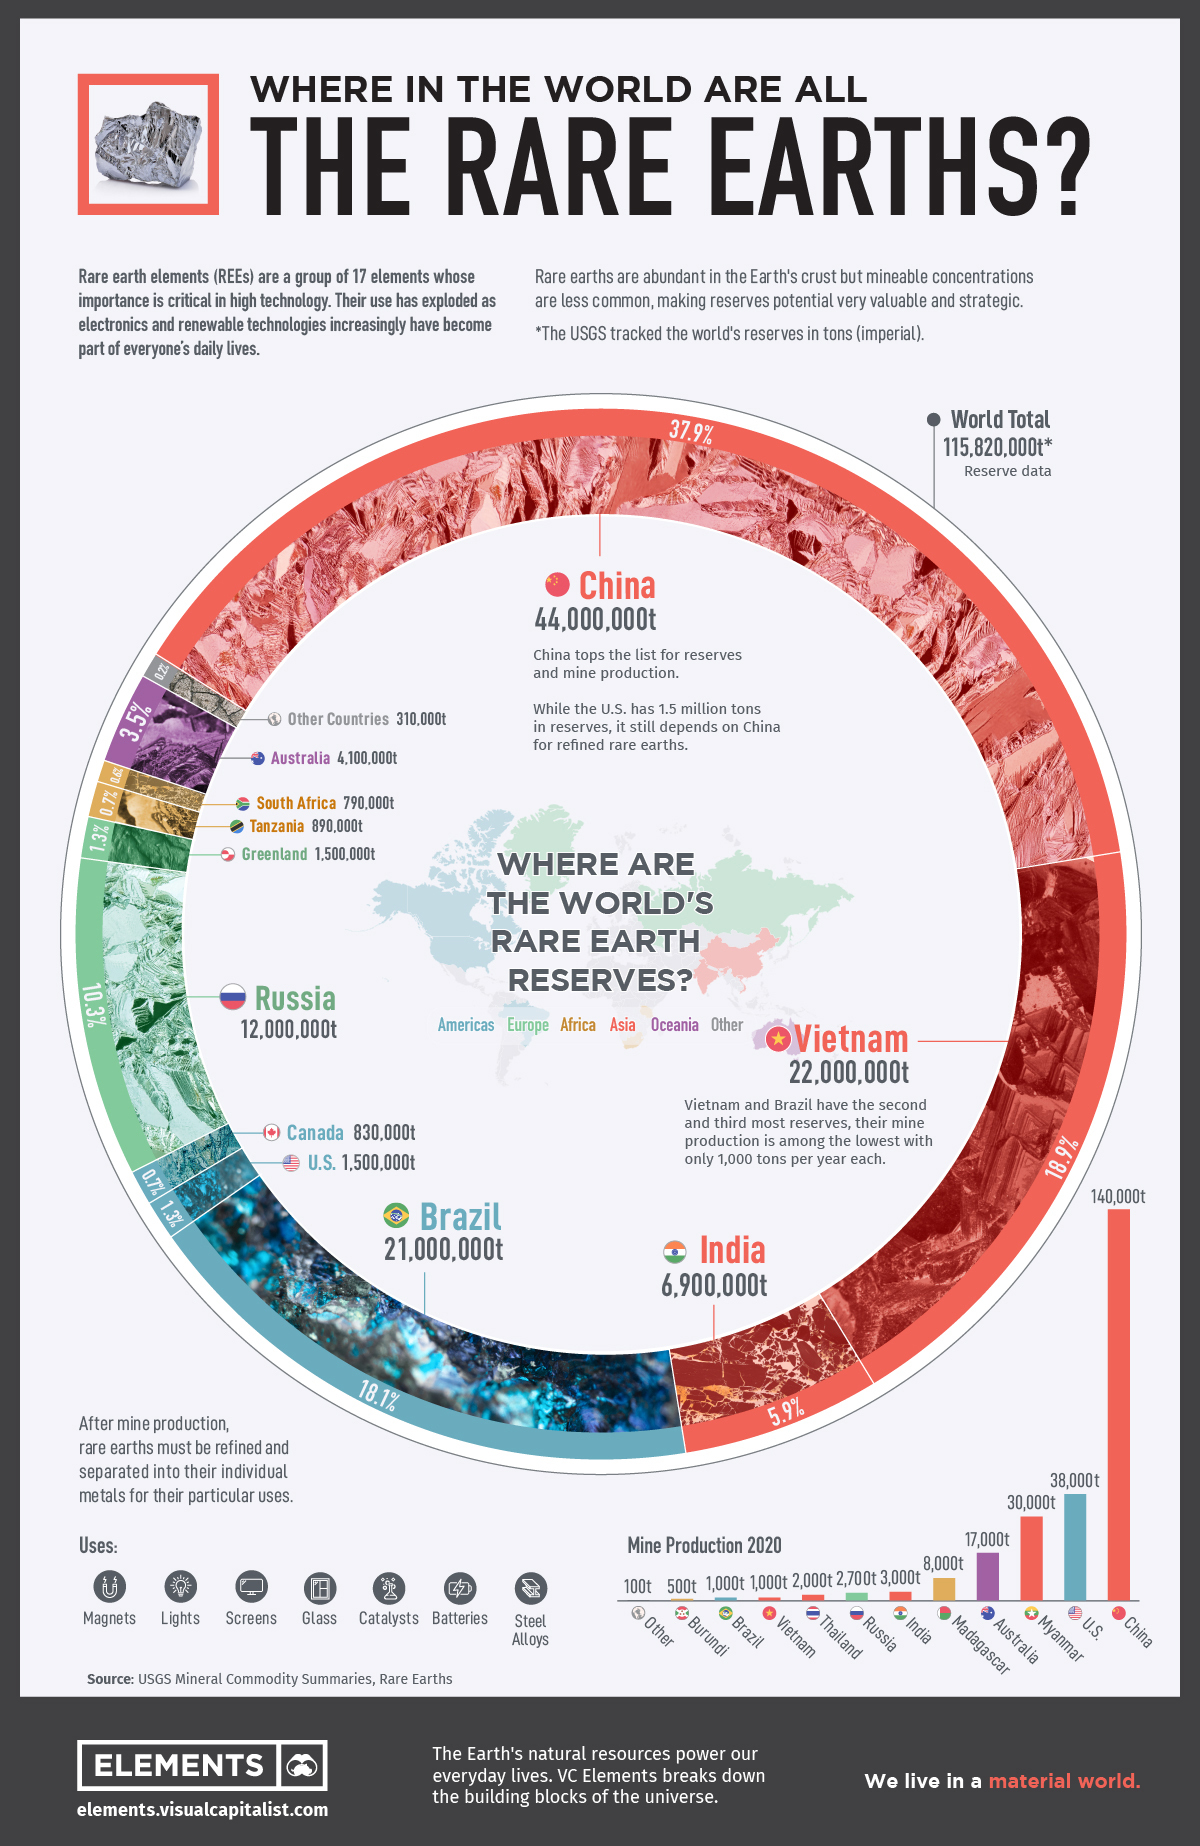
\includegraphics[width=0.42\textwidth]{pictures/rare-earths}
  \end{center}

\end{frame}

\begin{frame}{Peace and love?}

  \begin{center}
    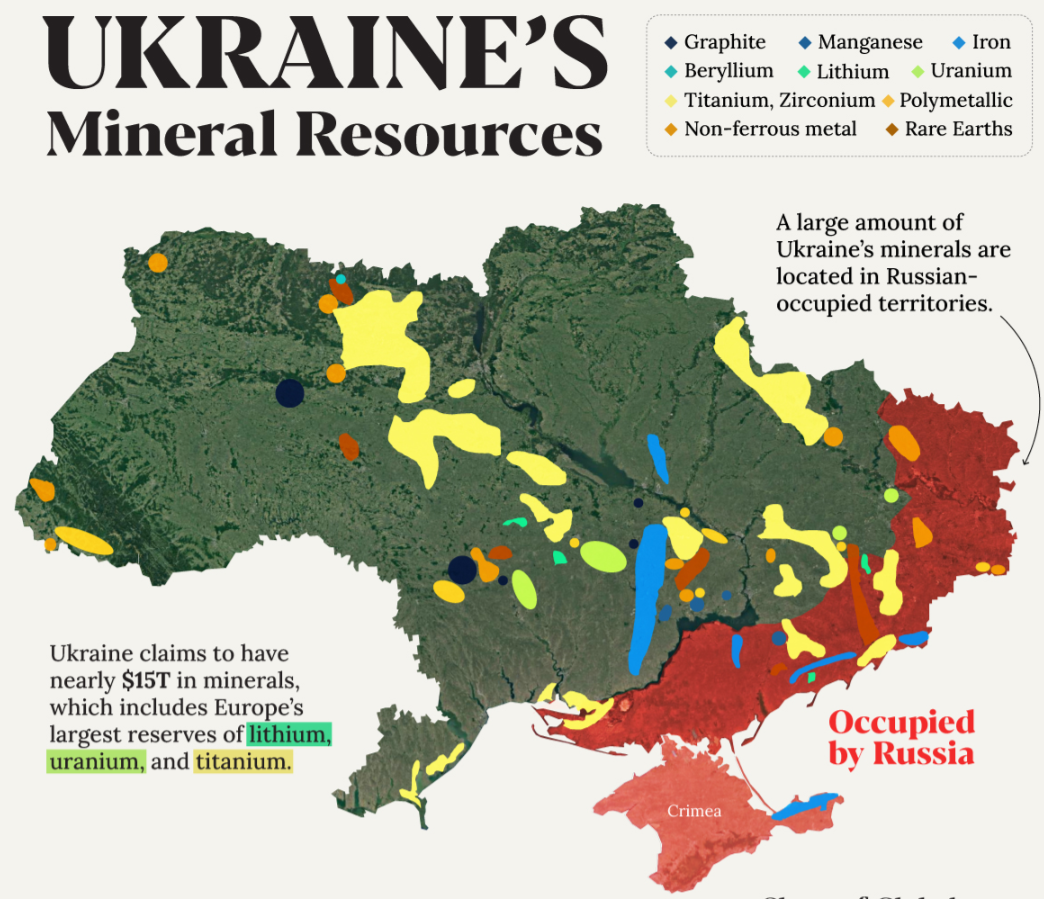
\includegraphics[width=0.7\textwidth]{pictures/ukraine}
  \end{center}

  \begin{center}
    {\tiny (source: \url{https://elements.visualcapitalist.com/mapped-ukraines-mineral-resources/})}
  \end{center}

\end{frame}

\begin{frame}{Peace and love?}

  \begin{center}
    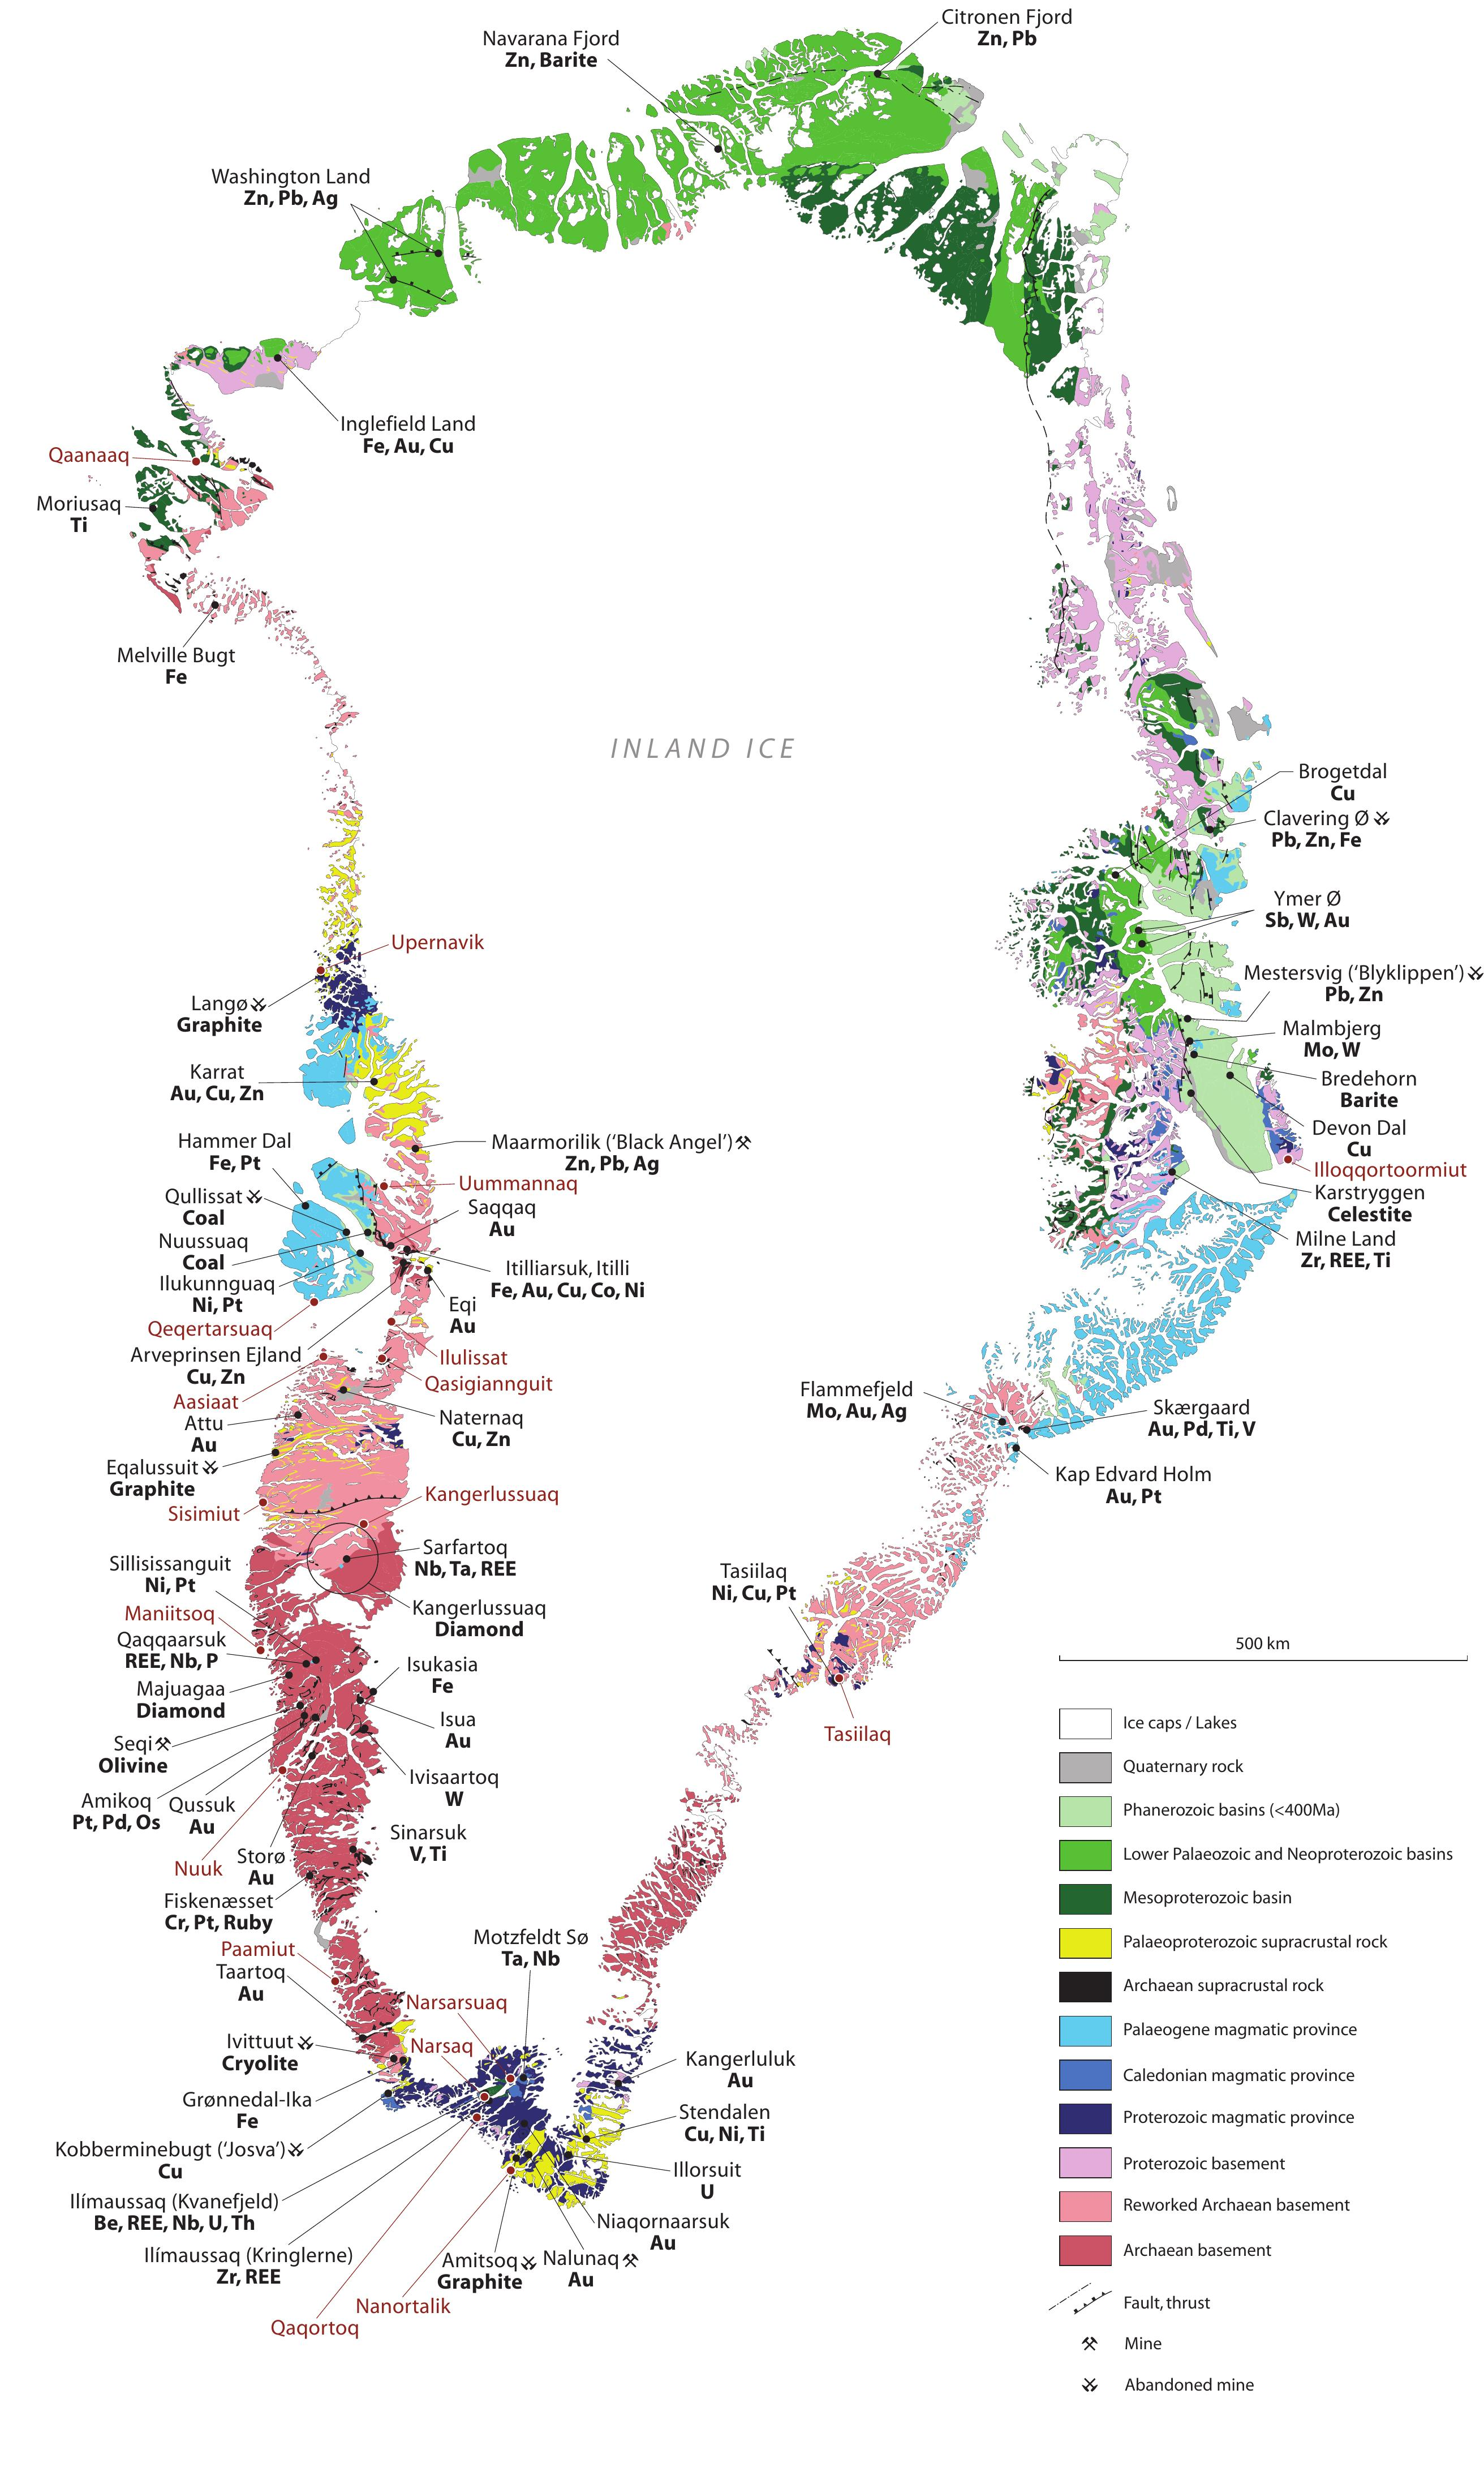
\includegraphics[width=0.35\textwidth]{pictures/greenland}
  \end{center}

  \begin{center}
    {\tiny (source: \url{https://www.academia.edu/20514876/Map_of_Greenland_geology_and_selected_mineral_occrrences})}
  \end{center}

\end{frame}

\begin{frame}{e-Waste}

  \begin{center}
    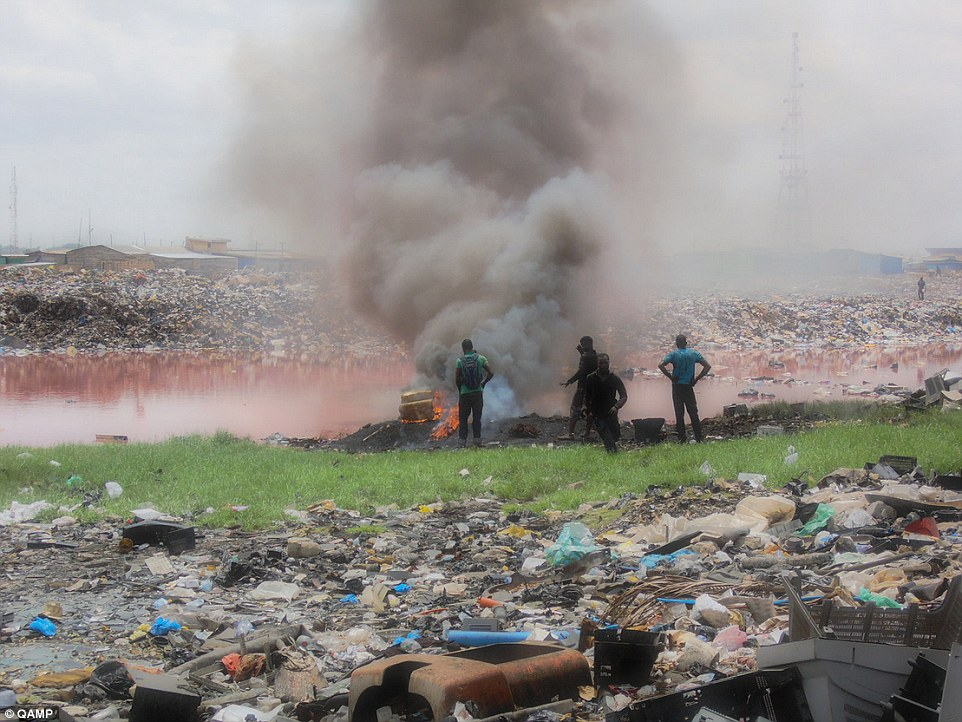
\includegraphics[width=0.7\textwidth]{pictures/e-waste}
  \end{center}

  \begin{center}
    Recycled, dumped, burned (mostly in poor countries)
  \end{center}

\end{frame}

\begin{frame}{Solutions?}

  Taming the ecological footprint of IT can only be achieved
  through a combined approach that integrates all its diverse aspects:

  \begin{itemize}
  \item technological advances
  \item social conscience
  \item political choices
  \end{itemize}

  \bigskip

  Let us dive deep inside Bitcoin to understand if we can do anything in the specific case
  of blockchain technology.

\end{frame}

\section{A more technical view of Bitcoin}

\begin{frame}{The blockchain peer-to-peer network}

  \begin{center}
    \begin{tikzpicture}[scale=0.5,>=Stealth]
      \draw[thick] (-10,0) -- (0,3.5) -- (10,0) -- cycle;

      \draw (-10,0) node[above=0.2] {\computer} node[below=0.2,fill=faustocolor] {Fausto};
      \only<2>{\draw (-7.5,1.7) node[above] {\leftArrow};}
      \only<2>{\draw (-6,2.5) node[above] {{\tiny\signature\ Alice $\xRightarrow{100}$ Donald}};}
      \draw (-10.5,3.5) rectangle +(1,0.5) [fill=gray!30!white];
      \draw[->] (-10,4.5) -- +(0,-0.5);
      \draw (-10.5,4.5) rectangle +(1,0.5) [fill=pink!70!white];
      \draw[->] (-10,5.5) -- +(0,-0.5); 
      \draw (-10.5,5.5) rectangle +(1,0.5) [fill=blue!30!white];
      \only<3->{\draw[->] (-10,6.5) -- +(0,-0.5); 
        \draw (-10.5,6.5) rectangle +(1,0.5) [fill=brown!70!white];}

      \draw (10,0) node[above=0.2] {\computer} node[below=0.2,fill=bobcolor] {Bob};
      \draw (9.5,3.5) rectangle +(1,0.5) [fill=gray!30!white];
      \draw[->] (10,4.5) -- +(0,-0.5);
      \draw (9.5,4.5) rectangle +(1,0.5) [fill=pink!70!white];
      \draw[->] (10,5.5) -- +(0,-0.5); 
      \draw (9.5,5.5) rectangle +(1,0.5) [fill=blue!30!white];
      \only<3->{\draw[->] (10,6.5) -- +(0,-0.5); 
        \draw (9.5,6.5) rectangle +(1,0.5) [fill=brown!70!white];}

      \draw[->] (0,3.5) node[above=0.2] {\computer} node[below=0.2,fill=alicecolor] {Alice};
      \only<4>{\filldraw [fill=gray!10!white] (0,8.25) circle [radius=1,very thick];}
      \only<2>{\draw (2.5,3.7) node[above] {\leftArrow};}
      \only<2>{\draw (4,4.5) node[above] {{\tiny\signature\ Donald $\xRightarrow{2500}$ John}};}
      \draw (-0.5,7) rectangle +(1,0.5) [fill=gray!30!white];
      \draw[->] (0,8) -- +(0,-0.5);
      \draw (-0.5,8) rectangle +(1,0.5) [fill=pink!70!white];
      \draw[->] (0,9) -- +(0,-0.5);
      \draw (-0.5,9) rectangle +(1,0.5) [fill=blue!30!white];
      \visible<3->{\draw[->] (0,10) -- +(0,-0.5); 
        \draw (-0.5,10) rectangle +(1,0.5) [fill=brown!70!white];}

    \end{tikzpicture}
  \end{center}

  \begin{center}
    \only<1>{Each peer holds a private copy of the same blockchain data structure.}
    \only<2>{Users can send signed transactions to any peer.}
    \only<3>{Such transactions get eventually boxed into new blocks.}
    \only<4>{Let us inspect a block of the blockchain.}
  \end{center}

\end{frame}

\begin{frame}{Blocks}
  \begin{center}
    \begin{tikzpicture}[scale=0.8]
      \visible<2->{\draw [decorate,decoration={brace,amplitude=4pt},thick,xshift=0.3cm,yshift=0pt]
        (4.5,7.5) -- (4.5,5.5) node [midway,right,xshift=.2cm] {trunk};}
      \only<1-13,15->{\draw [fill=VioletRed, thick] (0,6.5) rectangle +(4.5,1);}
      \only<14>{\shadedraw [inner color=VioletRed,outer color=white, draw=black, thick] (0,6.5) rectangle +(4.5,1);}
      \draw (2.25,7) node{height};
      \draw [fill=VioletRed, thick] (0,5.5) rectangle +(4.5,1);
      \visible<2->{\draw (2.25,6) node{$\pi$ (creator's key)};}
      \only<1-12,14->{\draw [fill=Yellow, thick] (0,4.5) rectangle +(4.5,1);}
      \only<13>{\draw [inner color=Yellow,outer color=white, draw=black, thick] (0,4.5) rectangle +(4.5,1);}
      \only<3->{\draw (2.25,5) node{$\previousblockhash$};}
      \only<-3>{\phantom{\draw[->,thick] (0,5) -- (-1,5) node [midway,left,xshift=-.5cm] {$\previous$};}}
      \only<3->{\draw[->,thick] (0,5) -- (-1,5) node [midway,left,xshift=-.5cm] {$\previous$};}

      \draw [fill=Yellow, thick] (0,3.5) rectangle +(4.5,1);
      \visible<4->{\draw (2.25,4) node{nonce\,(arbitrary data)};}

      \only<1-14,17->{\draw [fill=Yellow, thick] (0,2.5) rectangle +(4.5,1);}
      \only<15,16>{\draw [inner color=Yellow,outer color=white, draw=black, thick] (0,2.5) rectangle +(4.5,1);}
      \visible<5->{\draw (2.25,3) node{$\tau$ (creation time)};}

      \only<1-18>{\draw [fill=Yellow, thick] (0,1.5) rectangle +(4.5,1);}
      \only<19>{\draw [inner color=Yellow,outer color=white, draw=black, thick] (0,1.5) rectangle +(4.5,1);}
      \visible<11->{\draw (2.25,2) node{finalStateId};}

      \only<1-6,8-16,19>{\draw [fill=SpringGreen, thick] (0,-1) rectangle +(4.5,2.5);}
      \only<7,17,18>{\draw [inner color=SpringGreen,outer color=white, draw=black, thick] (0,-1) rectangle +(4.5,2.5);}
      \visible<6-7>{\draw (2.25,0.3) node{transactions};}
      \visible<8->{\draw (2.25,1) node{\signature\ Alice $\xRightarrow{100}$ Donald};}
      \visible<9->{\draw (2.25,0.4) node{\signature\ Fausto $\xRightarrow{500}$ John};}
      \visible<10->{\draw (2.25,-0.2) node{\signature\ Donald $\xRightarrow{350}$ Alice};}
      \visible<11->{\draw (2.25,-0.8) node{\signature\ Donald $\xRightarrow{2500}$ John};}
    \end{tikzpicture}
  \end{center}

  \begin{center}
    \only<1-6>{\phantom{Rule 2: $\previous$ actually exists (no dangling pointers)}}
    \only<7-11>{Let us inspect the list of transactions.}
    \only<12>{Valid blocks satisfy all \alert{consensus rules}:}
    \only<13>{\alert{Rule 1:} $\previous$ actually exists (no dangling pointers)}
    \only<14>{\alert{Rule 2:} The height increases: $\height=\previous.\height+1$}
    \only<15>{\alert{Rule 3:} The creation time increases: $\previous.\tau<\tau$}
    \only<16>{\alert{Rule 4:} The creation time is not in the future: $\tau\le\tau_\now$}
    \only<17>{\alert{Rule 5:} Each transaction is correctly signed by its sender}
    \only<18>{\alert{Rule 6:} Senders hold the money that they send}
    \only<19>{\alert{Rule 7:} $\finalstateid$ is derived from $\previous.\finalstateid$ and $\transactions$}
  \end{center}

\end{frame}

\begin{frame}{Each peer (Alice) can expand a \textbf{block} with a \textbf{next} block}

  \begin{center}
    \begin{tikzpicture}[scale=0.81]
      \draw (2,8) node{\textbf{block}};

      \draw [fill=VioletRed, thick] (0,5.5) rectangle (4,7.5);
      \draw (2,7) node{height};
      \draw [fill=VioletRed, thick] (0,4.5) rectangle (4,6.5);
      \draw (2,6) node{$\pi$ (creator's key)};

      \draw [fill=Yellow, thick] (0,4.5) rectangle (4,5.5);
      \draw (2,5) node{$\previousblockhash$};

      \draw [fill=Yellow, thick] (0,3.5) rectangle (4,4.5);
      \draw (2,4) node{nonce};

      \draw [fill=Yellow, thick] (0,2.5) rectangle (4,3.5);
      \draw (2,3) node{$\tau$ (creation time)};
      
      \draw [fill=Yellow, thick] (0,1.5) rectangle (4,2.5);
      \draw (2,2) node{$\finalstateid$};

      \draw [fill=SpringGreen, thick] (0,-1) rectangle (4,1.5);
      \draw (2,0.25) node{transactions};

      \visible<2->{
      \draw (9.5,8) node{\textbf{next}};
      \draw [fill=VioletRed, thick] (6,6.5) rectangle (13,7.5);
      \draw (9.5,7) node{height+1};
      }
      \visible<3->{
      \draw [fill=VioletRed, thick] (6,5.5) rectangle (13,6.5);
      \draw (9.5,6) node{Alice's public key};
      }
      \visible<4->{
      \draw [fill=Yellow, thick] (6,4.5) rectangle (13,5.5);
      \draw (9.5,5) node{$\hash(\mathbf{block})$};
      \draw[->,very thick] (6,5) -- (4,5);
      }

      \visible<5->{
      \draw [fill=Yellow, thick] (6,3.5) rectangle (13,4.5);
      \draw (9.5,4) node{42 (or 17, or 13, or your bday)};
      }
      \visible<6->{
      \draw [fill=Yellow, thick] (6,2.5) rectangle (13,3.5);
      \draw (9.5,3) node{$\tau_\now$};
      }

      \visible<9->{
      \draw [decorate,decoration={brace,amplitude=4pt},thick,xshift=0.3cm,yshift=0pt]
      (13,1.5) -- (13,-0.1) node [midway,right,xshift=.2cm] {$\xi$};
      \draw [decorate,decoration={brace,amplitude=4pt},thick,xshift=0.3cm,yshift=0pt]
      (13,7.5) -- (13,5.5) node [midway,right,xshift=.2cm] {$\xi$};
      \draw [decorate,decoration={brace,amplitude=4pt},thick,xshift=0.3cm,yshift=0pt]
      (13,3.5) -- (13,2.5) node [midway,right,xshift=.2cm] {$\xi$};
      \draw [fill=Yellow, thick] (6,1.5) rectangle (13,2.5);
      \draw (9.5,2) node{$\execute(\finalstateid,\xi)$};
      }

      \visible<7->{
      \draw [fill=SpringGreen, thick] (6,-1) rectangle (13,1.5);
      \draw (9.5,0.9) node{\signature\ Alice $\xRightarrow{100}$ Donald};
      \draw (9.5,0.15) node{\signature\ Donald $\xRightarrow{2500}$ John};
      }

      \visible<8->{
      \draw (9.5,-0.6) node{\textbf{ $\xRightarrow{432}$ Alice (implicit, coinbase)}};
      }
    \end{tikzpicture}
  \end{center}

\end{frame}

\begin{frame}{Peers create (``mine'') new blocks}

  \begin{center}
    \begin{tikzpicture}[scale=0.5,>=Stealth]

      \draw[thick] (-10,0) -- (0,3.5) -- (10,0) -- cycle;

      \draw (-10,0) node[above=0.2] {\computer} node[below=0.2,fill=faustocolor] {Fausto};
      \draw (-10.5,3.5) rectangle +(1,0.5) [fill=gray!30!white];
      \draw[->] (-10,4.5) -- +(0,-0.5);
      \draw (-10.5,4.5) rectangle +(1,0.5) [fill=pink!70!white];
      \draw[->] (-10,5.5) -- +(0,-0.5); 
      \draw (-10.5,5.5) rectangle +(1,0.5) [fill=blue!30!white];
      \visible<2-3,5,7-8,10>{\draw[->] (-10,6.5) -- +(0,-0.5);}
      \visible<9>{\draw[->] (-10.5,6.5) -- +(0.5,-0.5);}
      \visible<9>{\draw[->] (-9.5,6.5) -- +(-0.5,-0.5);}
      \visible<2-3,8>{\draw (-10.5,6.5) rectangle +(1,0.5) [fill=faustocolor];}
      \visible<5,10>{\draw (-10.5,6.5) rectangle +(1,0.5) [fill=alicecolor];}
      \visible<7>{\draw (-10.5,6.5) rectangle +(1,0.5) [fill=bobcolor];}
      \visible<9>{\draw (-11.2,6.5) rectangle +(1,0.5) [fill=faustocolor];}
      \visible<9>{\draw (-9.8,6.5) rectangle +(1,0.5) [fill=alicecolor];}

      \draw (10,0) node[above=0.2] {\computer} node[below=0.2,fill=bobcolor] {Bob};
      \draw (9.5,3.5) rectangle +(1,0.5) [fill=gray!30!white];
      \draw[->] (10,4.5) -- +(0,-0.5);
      \draw (9.5,4.5) rectangle +(1,0.5) [fill=pink!70!white];
      \draw[->] (10,5.5) -- +(0,-0.5); 
      \draw (9.5,5.5) rectangle +(1,0.5) [fill=blue!30!white];
      \visible<3,5-7,10>{\draw[->] (10,6.5) -- +(0,-0.5);}
      \visible<9>{\draw[->] (9.5,6.5) -- +(0.5,-0.5);}
      \visible<9>{\draw[->] (10.5,6.5) -- +(-0.5,-0.5);}
      \visible<3>{\draw (9.5,6.5) rectangle +(1,0.5) [fill=faustocolor];}
      \visible<5,10>{\draw (9.5,6.5) rectangle +(1,0.5) [fill=alicecolor];}
      \visible<6-7>{\draw (9.5,6.5) rectangle +(1,0.5) [fill=bobcolor];}
      \visible<9>{\draw (8.8,6.5) rectangle +(1,0.5) [fill=faustocolor];}
      \visible<9>{\draw (10.2,6.5) rectangle +(1,0.5) [fill=alicecolor];}

      \draw (0,3.5) node[above=0.2] {\computer} node[below=0.2,fill=alicecolor] {Alice};
      \draw (-0.5,7) rectangle +(1,0.5) [fill=gray!30!white];
      \draw[->] (0,8) -- +(0,-0.5);
      \draw (-0.5,8) rectangle +(1,0.5) [fill=pink!70!white];
      \draw[->] (0,9) -- +(0,-0.5);
      \draw (-0.5,9) rectangle +(1,0.5) [fill=blue!30!white];
      \visible<3-5,7-8,10>{\draw[->] (0,10) -- +(0,-0.5);}
      \visible<9>{\draw[->] (-0.5,10) -- +(0.5,-0.5);}
      \visible<9>{\draw[->] (0.5,10) -- +(-0.5,-0.5);}
      \visible<3>{\draw (-0.5,10) rectangle +(1,0.5) [fill=faustocolor];}
      \visible<4-5,8,10>{\draw (-0.5,10) rectangle +(1,0.5) [fill=alicecolor];}
      \visible<7>{\draw (-0.5,10) rectangle +(1,0.5) [fill=bobcolor];}
      \visible<9>{\draw (-1.2,10) rectangle +(1,0.5) [fill=faustocolor];}
      \visible<9>{\draw (0.2,10) rectangle +(1,0.5) [fill=alicecolor];}

    \end{tikzpicture}
  \end{center}

  \begin{overprint}
    \onslide<2-3>
    \centering Fausto creates a new block\ldots
    \onslide<4-5>
    \centering \ldots or Alice creates a new block
    \onslide<6-7>
    \centering \ldots or Bob creates a new block
    \onslide<8-9>
    \centering \ldots or Fausto and Alice create a new block!
    \onslide<10>
    \centering Peers select the block with the largest hash.
  \end{overprint}

\end{frame}

\begin{frame}{Blockchain mining as a competitive puzzle}

  Mining of a \textbf{next} block on top of a \textbf{block}:
  \quad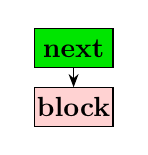
\begin{tikzpicture}[scale=0.5,>=Stealth]
    \draw (0,1.5) rectangle +(2,1) [fill=alicecolor];
    \draw[->] (1,1.5) -- +(0,-0.5);
    \draw (0,0) rectangle +(2,1) [fill=pink!70!white];
    \draw (1,0) node[above] {\textbf{block}};
    \draw (1,1.5) node[above] {\textbf{next}};
  \end{tikzpicture}

  \begin{description}
  \item[{\color{red}challenge:}] \only<2->{derive (deterministically) a challenge from the \textbf{block}}
  \item[{\color{red}answer:}] \only<3->{send all peers a \textbf{next} that satisfies the challenge}
  \item[{\color{red}competition:}] \only<4->{in case of more \textbf{next}, select a \emph{best} one}
  \end{description}

  \bigskip
  \visible<5->{Bitcoin's Proof of Work (PoW):}
  \begin{description}
  \item<6->[{\color{red}challenge:}] find a valid \textbf{next} of \textbf{block}
    such that $\hash(\mathbf{next})\ge\difficulty$
  \item<7->[{\color{red}answer:}] send all peers a \textbf{next} obtained
    by rotating among possible values for its nonce, until $\hash(\mathbf{next})\ge\difficulty$
  \item<8->[{\color{red}competition:}] in case of more \textbf{next}, select the one with the largest hash
  \end{description}

\end{frame}

\begin{frame}[fragile]{Bitcoin's proof of work mining is brute force}
 
\begin{algorithm}[H] 
\caption{Bitcoin's Proof of Work}
\begin{algorithmic}[1]
\Require{$block$, $difficulty$, $max$} 
\Ensure{$next$ (a valid child of $block$, or null)}
\Statex
\State {$next$ $\gets$ null}
\For{$nonce \gets 0$ to $max$}
\State {$candidate$ $\gets$ valid next of block that uses $nonce$}
\If{hash($candidate$) $\ge$ $difficulty$}
\If{$next$ = null \textbf{or} hash($candidate$) $>$ hash($next$)}
\State {$next$ $\gets$ $candidate$}
\EndIf
\EndIf
\EndFor
\State \Return {$next$}
\end{algorithmic}
\end{algorithm} 

\end{frame}

\begin{frame}\frametitle{The magic behind the proof of work}

  \begin{greenbox}{}
    It makes expensive the production of new blocks, in time and cost (electricity)
    \begin{itemize}
    \item who produces invalid blocks sees its blocks rejected by peers and wastes resources
    \item a single node cannot dictate the history easily, since it must fight against
      the hashing power of all other nodes together
    \item forks become unlikely, since the probability of two nodes finding a new block at the same time is small
    \end{itemize}
  \end{greenbox}

\end{frame}

\begin{frame}\frametitle{Evolution of Bitcoin's mining hardware}

  \begin{center}
    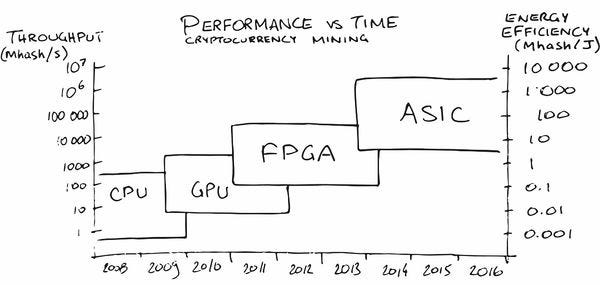
\includegraphics[scale=0.55,clip=false]{pictures/mining-hardware}
  \end{center}

\end{frame}

\begin{frame}\frametitle{Bitcoin's difficulty over the years}

  \begin{center}
    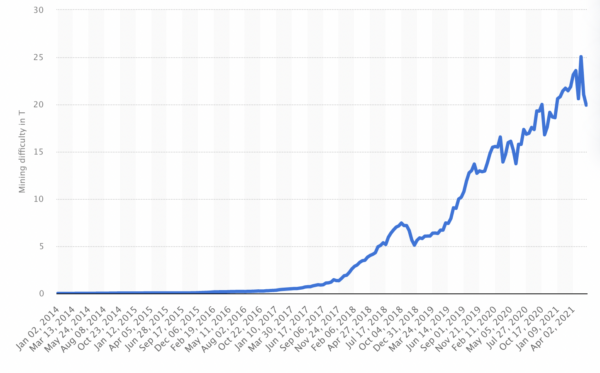
\includegraphics[width=0.9\textwidth,clip=false]{pictures/difficulty}
  \end{center}

  \begin{center}
    {\tiny (source: \url{https://thresh0ld.com/bitcoin-mining-difficulty-and-price-correlation})}
  \end{center}
    
\end{frame}

\part{2}

\section{The proof of stake alternative}

\begin{frame}\frametitle{The proof of stake alternative to proof of work}

  \begin{center}
    Jae Kwon, \emph{Tendermint, Consensus without Mining}, 2014
  \end{center}

  \begin{greenbox}{}
    A selected set of peers (\emph{validators}) decides the next block, in
    a round robin way or according to any other \emph{fair} policy, typically
    based on the amount of money \emph{staked} by each validator.
    Byzantine algorithms ensure the survival of the peer-to-peer network if
    \emph{some} validators misbehave.

    \begin{itemize}
    \item proof of work: all peers are created equal
    \item proof of stake: but some peers are more equal than others
    \end{itemize}
  \end{greenbox}

  \medskip

  \pause

  \begin{center}
    Pros: no CPU mining anymore, higher throughput
  \end{center}

  \begin{center}
    Cons: more centralized, the rich become richer
  \end{center}

  \medskip

  \begin{center}
    $99\%$ of cryptocurrencies are based on proof of stake nowadays.
  \end{center}

  \pause

  \begin{center}
    \alert{Are Bitcoin and its proof of work dead then?}
  \end{center}

\end{frame}

\begin{frame}{It's the economy, stupid!}

  \begin{center}
    Bitcoin (proof of work) to USD\\
    \vspace*{1ex}
    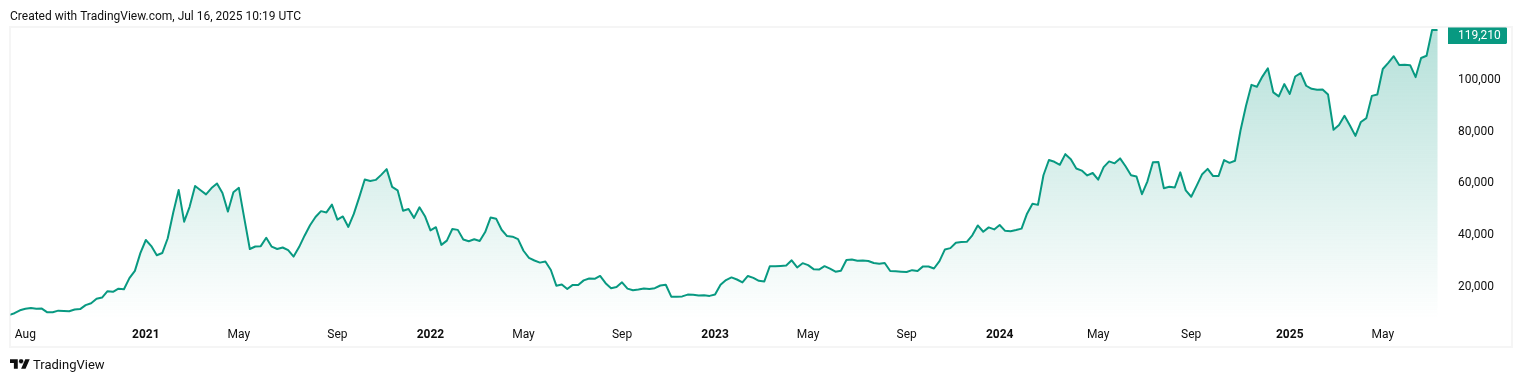
\includegraphics[width=\textwidth]{pictures/BTCUSD}
  \end{center}

  \medskip

  \begin{overprint}
    \onslide<2>
    \begin{center}
      Ethereum (proof of stake) to USD\\
      \vspace*{1ex}
      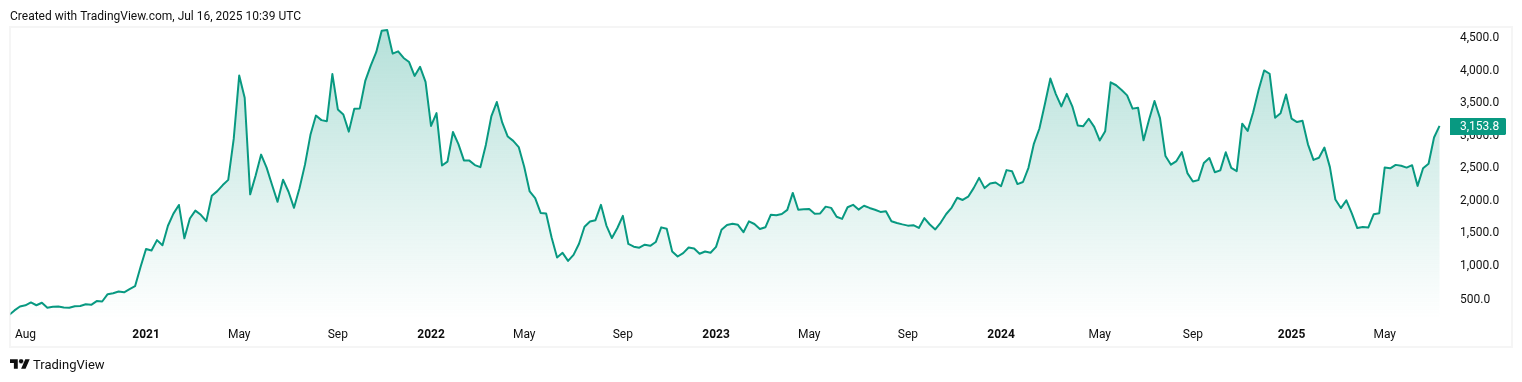
\includegraphics[width=\textwidth]{pictures/ETHUSD}
    \end{center}
    \onslide<3>
    \begin{center}
      Solana (proof of stake) to USD\\
      \vspace*{1ex}
      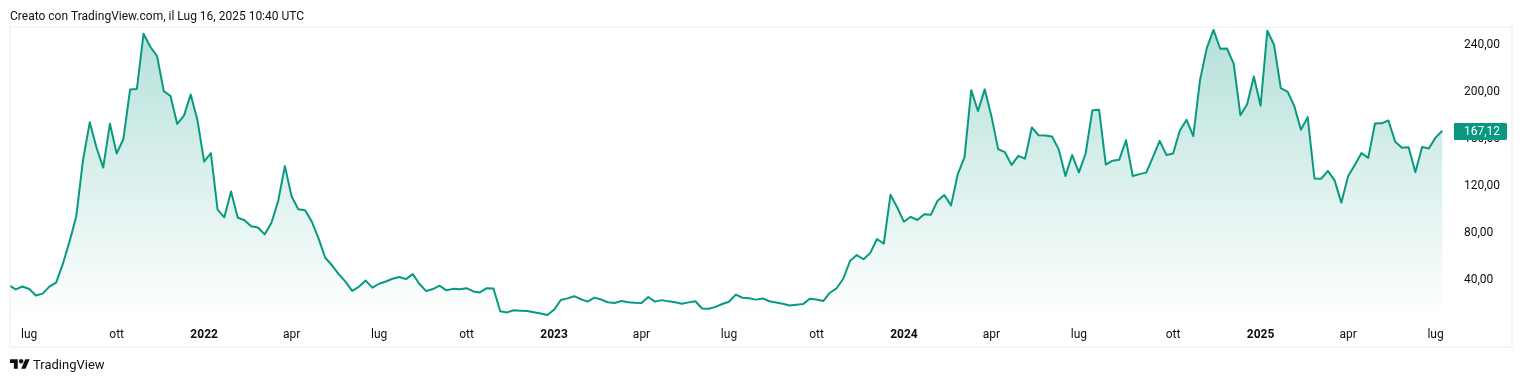
\includegraphics[width=\textwidth]{pictures/SOLUSD}
    \end{center}
    \onslide<4>
    \begin{center}
      Cardano (proof of stake) to USD\\
      \vspace*{1ex}
      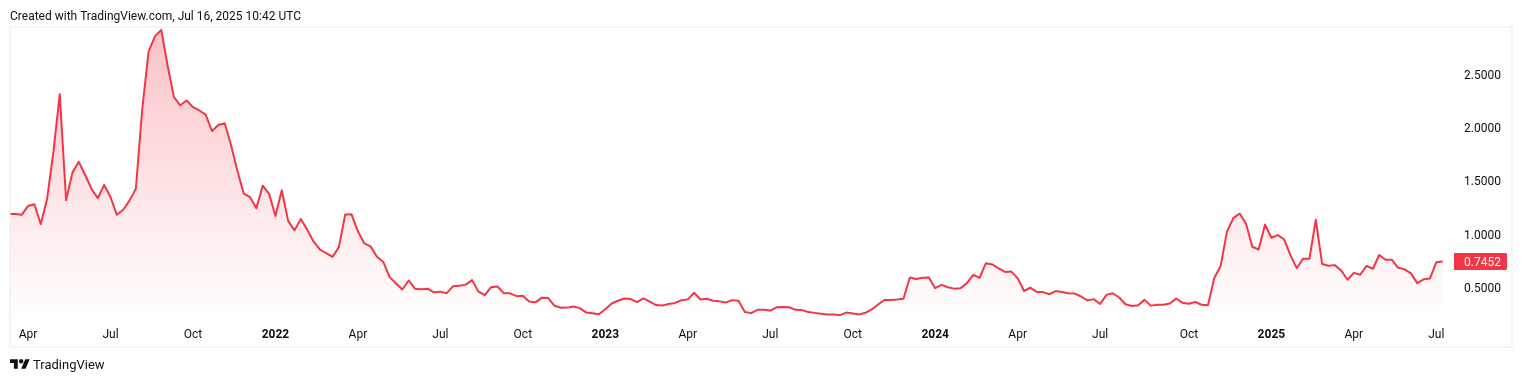
\includegraphics[width=\textwidth]{pictures/ADAUSD}
    \end{center}
    \onslide<5>
    \begin{center}
      Polygon (proof of stake) to USD\\
      \vspace*{1ex}
      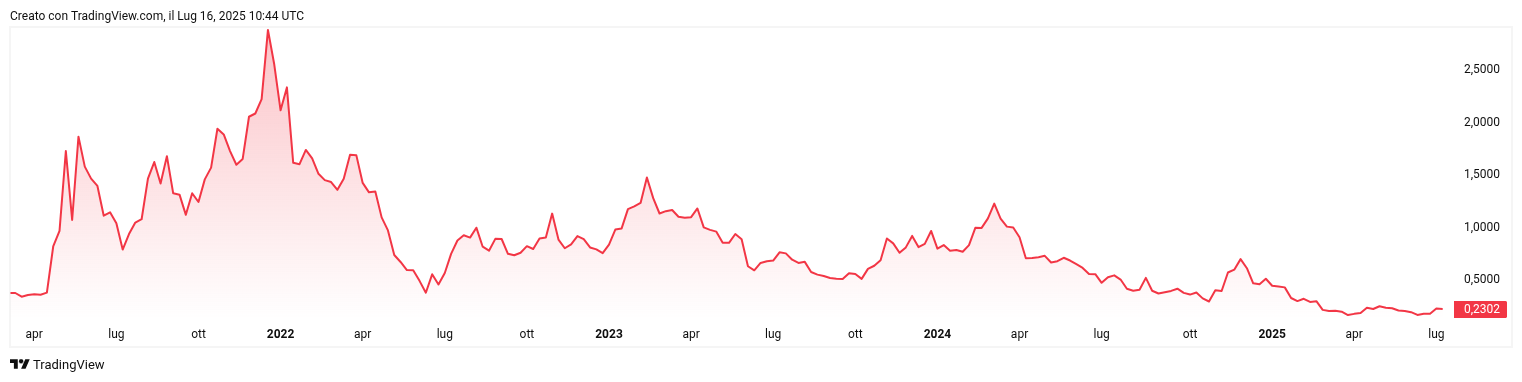
\includegraphics[width=\textwidth]{pictures/MATICUSD}
    \end{center}
    \centering \ldots or Fausto and Alice create a new block!
    \onslide<6>
    \begin{center}
      Dogecoin (proof of stake) to USD\\
      \vspace*{1ex}
      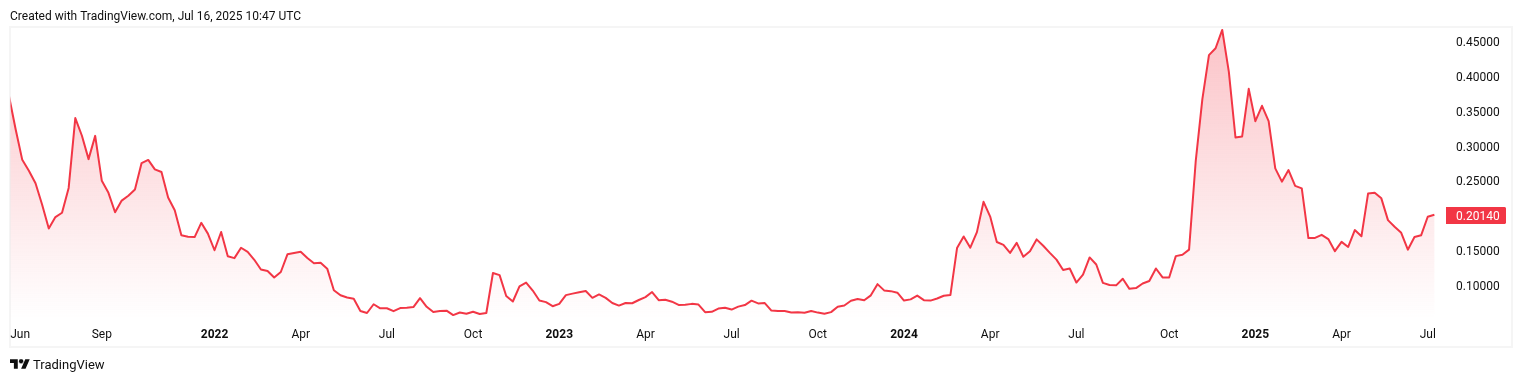
\includegraphics[width=\textwidth]{pictures/DOGEUSD}
    \end{center}
  \end{overprint}

\end{frame}

\begin{frame}{Looking for the chimera}

  \begin{center}
    As decentralized as Bitcoin's proof of work, as cheap as proof of stake
  \end{center}

  \medskip

  \begin{center}
    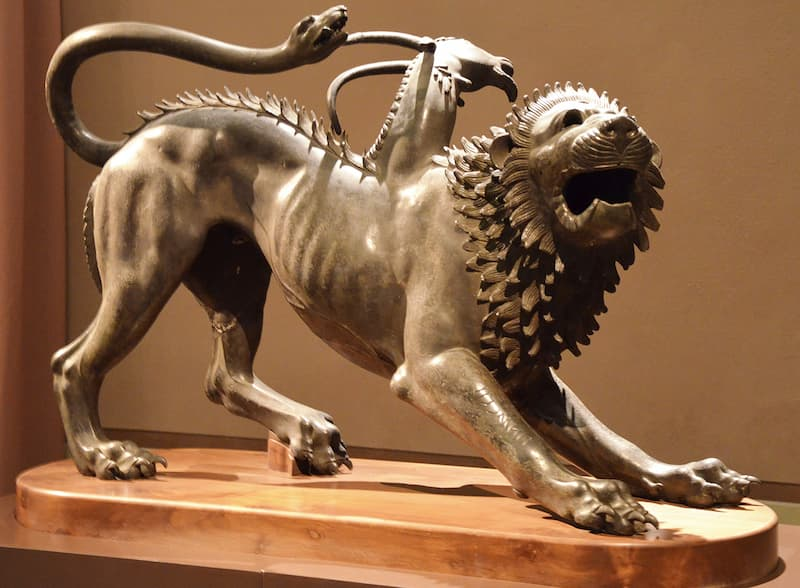
\includegraphics[width=0.7\textwidth]{pictures/chimera}\\
    {\tiny Florence, Etruscan chimera, 400 BC}
  \end{center}

\end{frame}

\section{The proof of space alternative}

\begin{frame}{An email from \texttt{crypto42@pm.me} (September 30, 2021)}

  \begin{greenbox}{}
    Hi Fausto!

    \vspace{2ex}

    I have been experimenting with a blockchain called \alert{Signum: \url{https://signum.network/}}.
    They \alert{mine with
    disk drive files (plot files)}, which is far more at reach
    and \alert{ecological} than GPUs or CPUs.

    \vspace{1ex}

    I've been trying with other developers to make their mining 100\%
    Java based. This would open the door for end-users to easily \alert{mine directly
    from their cellphones} or from low-powered devices fueled by \alert{green energy}.
    Unfortunately that was beyond our skills.

    \vspace{1ex}

    I saw your Hotmoka smart contracts project on GitHub.
    I wonder if disk drive mining, also on cell phones, can be achieved with Hotmoka.
  \end{greenbox}

\end{frame}

\begin{frame}{What I could learn about Signum}

  \begin{itemize}
  \item very simple protocol for proof of space (PoSp)
  \item recently, proof of space + proof of commitment
    \begin{itemize}
    \item[] just a factor multiplication of proof of space
      based on the committed cryptocurrency, as an incentive
      to buying their cryptocurrency
    \end{itemize}
  \item running since 2014 (as Burstcoin)
  \item possibly the first ever smart contracts (before Ethereum!)
  \item commercial web page: \url{https://signum.network/}
  \item very informal documentation:
    \url{https://wiki.signum.network}
  \item chaotic, uncommented, monolithic code:
    \url{https://github.com/signum-network/signum-node}
  \item Park et al., \emph{SpaceMint: A Cryptocurrency Based on Proofs of Space},
    Financial Cryptography 2018,
    show that Signum originally suffered from a time/memory tradeoff
    and suspect that it suffers from block-grinding attacks as well
  \end{itemize}

\end{frame}

\begin{frame}\frametitle{Proof of space is much more than Signum}

  \begin{greenbox}{}
    \begin{itemize}
    \item Ateniese, Bonacina, Faonio, Galesi: \emph{Proofs of Space: When Space Is of the Essence}, 2014 (DAG pebbling)
    \item Dziembowski, Faust, Kolmogorov, Pietrzak: \emph{Proofs of Space}, 2015 (DAG pebbling) $\Rightarrow$
      {\color{red}SpaceMint}: \url{https://github.com/kwonalbert/spacemint}
    \item Abusalah, Alwen, Cohen, Khilko, Pietrzak, Reyzin: \emph{Beyond Hellman's Time-Memory Trade-Offs with Applications to Proofs of Space}, 2017 (proof of sequential work + proof of space) $\Rightarrow$ {\color{red}Chia}: \url{https://www.chia.net/wp-content/uploads/2022/07/ChiaGreenPaper.pdf}
    \end{itemize}

  \begin{center}
    {\small\begin{tabular}{c|c|c|c|c|c}
      tool & consensus & network & formalized & since & status \\\hline\hline
      SpaceMint & no & no & yes & 2015 & discontinued\\\hline
      Chia & yes & yes & yes & 2017 & active\\\hline
      Signum & yes & yes & no & 2014 & active\\\hline
    \end{tabular}}
  \end{center}
  \end{greenbox}
  
\end{frame}

\begin{frame}\frametitle{Proof of space: The general idea}

  \begin{description}
  \item[Ideal PoSp:] the computation of the answer can only be achieved by allocating
    a big data structure on disk (Ateniese et al., Dziembowski et al., Abusalah et al.)
    \medskip
  \item[Signum's PoSp:] the computation of the answer can be achieved with or without
    allocating a big data structure on disk (precomputed \emph{nonces}),
    but in the latter case it becomes
    computationally so expensive (to recompute the data on-the-fly)
    that the space of explorable data, before the next block is created, is very small
  \end{description}

  \bigskip
  
  \begin{redbox}{Time/memory trade-off}
    The degradation of the space of explorable data should be at least linear with
    the reduction of the precomputed data.
  \end{redbox}

\end{frame}

\begin{frame}\frametitle{Signum's proof of space}

  \visible<1->{Blocks use a $\nonce$ data structure of size $n$ and creator $\pi$.}
  \medskip

  \begin{description}
  \item<2->[{\color{red}challenge:}] given a $\challenge$
    derived from \textbf{block}, find a valid \textbf{next} of \textbf{block}
    with a $\nonce$ data structure for the same creator of the block,
    such that $\delay(\nonce,\challenge)$ is as smaller as possible
  \item<3->[{\color{red}answer:}] reply with a valid \textbf{next} of \textbf{block}
    that contains a $\nonce$ from
    a large set of nonces precomputed on disk,
    choosing the one that minimizes $\delay(\nonce,\challenge)$
    and using, as block's creator, the same creator of $\nonce$
  \item<4->[{\color{red}competition:}] in case of more \textbf{next}, select the one with the smallest
    $\delay(\nonce,\challenge)$
  \end{description}

\end{frame}

\begin{frame}{A work of formalization}

  A formalization of Signum's proof of space requires to clarify:
  \begin{description}
  \item[Point~1:] what is the nonce data structure
  \item[Point~2:] how a challenge is derived from a block
  \item[Point~3:] how $\delay(\nonce,\challenge)$ is defined
  \end{description}

  \pause

  \medskip

  Once a formalization is available, it can be used to \alert{prove} that
  the algorithm is immune from some typical attacks and as the basis for
  a clean implementation.

  \bigskip

  \begin{greenbox}{}
    Fausto Spoto, \emph{A Formalization of Signum Consensus},
    Financial Cryptography Workshop on Trusted Smart Contracts,
    Miyakojima, Japan, 2025, To appear in LNCS.
  \end{greenbox}

\end{frame}

\begin{frame}{Point~1: The nonce data structure}
  \begin{center}
    $p\in\mathbb{N}$ (\emph{progressive}) and $\pi\in\mathit{byte}^*$ (at least the public key of the creator)
  \end{center}
  \[\begin{array}{l}
  \pause
  \seed=\pi\bowtie p\quad\text{($\bowtie$ is byte array concatenation)}\\
  \pause
  {\color{blue} h_0}=\hashfirstk(\seed)\\
  \pause
  {\color{blue} h_1}=\hashfirstk({\color{blue} h_0}\bowtie\seed)\\
  \pause
  {\color{blue} h_2}=\hashfirstk({\color{blue} h_1}\bowtie{\color{blue}  h_0}\bowtie \seed)\\
  \pause
  \vdots\\
  {\color{blue} h_{2n-1}}=\hashfirstk({\color{blue} h_{2n-2}}\bowtie{\color{blue} h_{2n-3}}\bowtie\cdots\bowtie{\color{blue} h_1}\bowtie{\color{blue} h_0}\bowtie \seed)\\
  \pause
  {\color{red}\finalhash}=\hash({\color{blue} h_{2n-1}}\bowtie{\color{blue} h_{2n-2}}\bowtie\cdots\bowtie{\color{blue} h_1}\bowtie{\color{blue} h_0}\bowtie \seed)\\
  \pause
  \text{reassign }{\color{blue} h_i}={\color{blue} h_i}\oplus{\color{red}\finalhash}\text{ for every }0\le i<2n\quad\text{($\oplus$ is byte array xor)}\\
  \end{array}\]

  \pause

  \[
  \nonce(p,\pi)=\langle p,\pi,\underbrace{\underbrace{{\color{blue}h_0},{\color{blue}h_{2n-1}}}_{\scoop_0},\underbrace{{\color{blue}h_2},{\color{blue}h_{2n-3}}}_{\scoop_1},\ldots,\underbrace{{\color{blue}h_{2n-4}},{\color{blue}h_3}}_{\scoop_{n-2}},\underbrace{{\color{blue}h_{2n-2}},{\color{blue}h_1}}_{\scoop_{n-1}}}_{\text{precomputed information, expensive to recompute on the fly}}\rangle
  \]

  \begin{overprint}
    \onslide<10>
    \centering hash is the expensive shabal256
    \onslide<11>
    \centering $\kappa$ allows one to modulate the cost of the computation
    \onslide<12>
    \centering $\scoop_i={\color{blue}h_{2i}},{\color{blue}h_{2n-2i-1}}$ depends from at least a ${\color{blue}h_j}$ with $j\ge n$
  \end{overprint}

\end{frame}

\begin{frame}[fragile]{Point~2: Derivation of a challenge from a block}

  \begin{align*}
    {\color{blue}\challenge(\genesis)}&=\langle 0,\sigma_\genesis\rangle,\quad\sigma_\genesis\text{ is an arbitrary byte array}\\
    \mbox{}\\
    \visible<2->{
    {\color{blue}\challenge(\block)}&=\langle\hash(\sigma\bowtie{\color{red}\height})\ \mathit{mod}\ n,\sigma\rangle\\
    &\text{where $\sigma=\hash({\color{blue}\challenge(\previous)}.\sigma\bowtie{\color{red}\pi})$}}
  \end{align*}

  \visible<2->{
  \begin{center}
    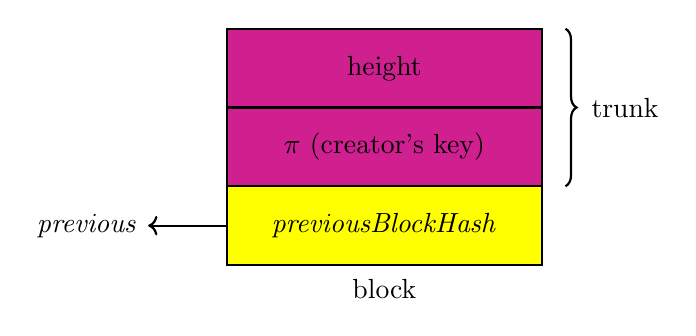
\begin{tikzpicture}
      \draw [decorate,decoration={brace,amplitude=4pt},thick,xshift=0.3cm,yshift=0pt]
      (4,7.5) -- (4,5.5) node [midway,right,xshift=.2cm] {trunk};
      \draw [fill=VioletRed, thick] (0,5.5) rectangle (4,7.5);
      \draw (2,7) node{height};
      \draw [fill=VioletRed, thick] (0,4.5) rectangle (4,6.5);
      \draw (2,6) node{$\pi$ (creator's key)};
      \draw [fill=Yellow, thick] (0,4.5) rectangle (4,5.5);
      \draw (2,5) node{$\previousblockhash$};
      \draw[->,thick] (0,5) -- (-1,5) node [midway,left,xshift=-.5cm] {$\previous$};
      \draw (2,4.2) node{block};
    \end{tikzpicture}
  \end{center}
  }

  \visible<3->{
  \begin{center}
    \textbf{Proposition.} Challenges depends on the trunks only (simple proof by induction): Signum has no block-grinding attacks.
  \end{center}
  }

\end{frame}

\begin{frame}{Point~3: The delay of a nonce \wrt a challenge}

  \begin{center}
  Let $\challenge={\color{blue}\langle i,\sigma\rangle}$ and
  $\nonce=\langle p,\pi,\underbrace{h_0,h_{2n-1}}_{\scoop_0},\underbrace{h_2,h_{2n-3}}_{\scoop_1},\ldots,\underbrace{h_{2n-4},h_3}_{\scoop_{n-2}},\underbrace{h_{2n-2},h_1}_{\scoop_{n-1}}\rangle$:
  \end{center}
  \bigskip
  \[
    \delay(\nonce,\challenge)=\hash(\scoop_{\color{blue}i}\bowtie{\color{blue}\sigma})
  \]

\end{frame}

\begin{frame}[fragile]{Signum's proof of space mining}
 
\begin{algorithm}[H] 
\caption{Signum's Proof of Space}
\begin{algorithmic}[1]
\Require{$block$, non-empty $plot$ file created by $\pi$}
\Ensure{$next$ (a valid child of $block$)}
\Statex
\State {$best\_nonce$ $\gets$ first nonce of $plot$}
\State {$c$ $\gets$ $\challenge(block)$}
\For{$nonce \in plot$}
\If{$\delay(nonce, c)$ $<$ $\delay(best\_nonce, c)$}
\State {$best\_nonce$ $\gets$ $nonce$}
\EndIf
\EndFor
\State \Return {valid $next$ of $block$, created by $\pi$ and using $best\_nonce$}
\end{algorithmic}
\end{algorithm} 

\end{frame}

\begin{frame}{Miner $\pi$ selects its $\bestNonce$ and builds a next block}

  \begin{center}
    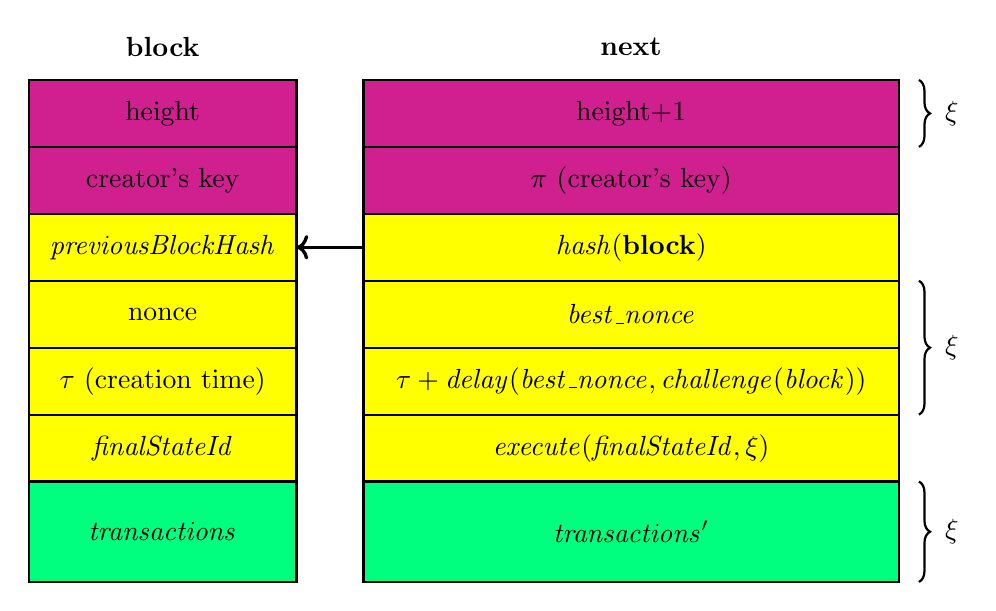
\begin{tikzpicture}[scale=0.85]
      \draw (2,8) node{\textbf{block}};
      \draw [fill=VioletRed, thick] (0,5.5) rectangle (4,7.5);
      \draw (2,7) node{height};
      \draw [fill=VioletRed, thick] (0,4.5) rectangle (4,6.5);
      \draw (2,6) node{creator's key};
      \draw [fill=Yellow, thick] (0,4.5) rectangle (4,5.5);
      \draw (2,5) node{$\previousblockhash$};

      \draw [fill=Yellow, thick] (0,3.5) rectangle (4,4.5);
      \draw (2,4) node{nonce};

      \draw [fill=Yellow, thick] (0,2.5) rectangle (4,3.5);
      \draw (2,3) node{$\tau$ (creation time)};

      \draw [fill=Yellow, thick] (0,1.5) rectangle (4,2.5);
      \draw (2,2) node{$\finalstateid$};

      \draw [fill=SpringGreen, thick] (0,0) rectangle (4,1.5);
      \draw (2,0.75) node{$\transactions$};

      \visible<2->{
      \draw (9,8) node{\textbf{next}};
      \draw [fill=VioletRed, thick] (5,6.5) rectangle (13,7.5);
      \draw (9,7) node{height+1};
      }
      \visible<3->{
      \draw [fill=VioletRed, thick] (5,5.5) rectangle (13,6.5);
      \draw (9,6) node{$\pi$ (creator's key)};
      }
      \visible<4->{
      \draw [fill=Yellow, thick] (5,4.5) rectangle (13,5.5);
      \draw (9,5) node{$\hash(\mathbf{block})$};
      \draw[->,very thick] (5,5) -- (4,5);
      }

      \visible<5->{
      \draw [fill=Yellow, thick] (5,3.5) rectangle (13,4.5);
      \draw (9,4) node{$\bestNonce$};
      }

      \visible<6->{
      \draw [fill=Yellow, thick] (5,2.5) rectangle (13,3.5);
      \draw (9,3) node{$\tau+\delay(\bestNonce,\challenge(\block))$};
      }

      \visible<8->{
        \draw [decorate,decoration={brace,amplitude=4pt},thick,xshift=0.3cm,yshift=0pt]
        (13,1.5) -- (13,0) node [midway,right,xshift=.2cm] {$\xi$};
        \draw [decorate,decoration={brace,amplitude=4pt},thick,xshift=0.3cm,yshift=0pt]
        (13,4.5) -- (13,2.5) node [midway,right,xshift=.2cm] {$\xi$};
        \draw [decorate,decoration={brace,amplitude=4pt},thick,xshift=0.3cm,yshift=0pt]
        (13,7.5) -- (13,6.5) node [midway,right,xshift=.2cm] {$\xi$};
        \draw [fill=Yellow, thick] (5,1.5) rectangle (13,2.5);
        \draw (9,2) node{$\execute(\finalstateid,\xi)$};
      }

      \visible<7->{
      \draw [fill=SpringGreen, thick] (5,0) rectangle (13,1.5);
      \draw (9,0.75) node{$\transactions'$};
      }
    \end{tikzpicture}
  \end{center}

\end{frame}

\begin{frame}{The life of a blockchain peer}

  A blockchain peer computer holds:
  \begin{itemize}
  \item a blockchain $B$
  \item a set of nonces precomputed on disk, called $\plot$
  \item a network connection to some other peers
  \end{itemize}

  \bigskip
  \pause
  It performs two algorithms concurrently:
  \begin{enumerate}
    \pause
  \item the block mining algorithm (produce blocks and send them to peers)
    \pause
  \item the block mined algorithm (receive blocks from peers and check them)
  \end{enumerate}

\end{frame}

\begin{frame}{The block mining algorithm}

  \begin{greenbox}{An infinite loop}
    \begin{enumerate}[<+->]
    \item\label{step:block_mining:loop} identify a most powerful $\mathbf{block}\in B$
    \item\label{step:block_mining:next_challenge} compute $c=\challenge(\mathbf{block})$
    \item\label{step:block_mining:next_deadline} select a nonce $\nu$ in $\plot$ that minimizes $\delay(\nu,c)$
    \item\label{step:block_mining:next_block} build block \textbf{next} by using $\nu$
    \item\label{step:block_mining:wait} wait until $\mathbf{next}.\tau\le\tau_\now$
    \item\label{step:block_mining:add} add $\mathbf{next}$ to $B$ [no check: consensus holds for \textbf{next} by construction]
    \item\label{step:block_mining:whisper} whisper $\mathbf{next}$ to the connected peers
    \item go back to step~\ref{step:block_mining:loop}
    \end{enumerate}
  \end{greenbox}

\end{frame}

\begin{frame}{The block mined algorithm}

  \begin{greenbox}{An infinite loop}
    \begin{enumerate}[<+->]
    \item\label{step:block_mined:loop} wait for a \textbf{block} whispered from some connected peer
    \item\label{step:block_mined:add} if $B\cup\{\mathbf{block}\}$ satifies consensus, add $\mathbf{block}$ to $B$ [consensus check: peers might be cheating]
    \item go back to step~\ref{step:block_mined:loop}
    \end{enumerate}
  \end{greenbox}

\end{frame}

\section{Mokamint and Hotmoka}

\begin{frame}{Mokamint (Fausto Spoto, 2023--2025)}

  \begin{center}
    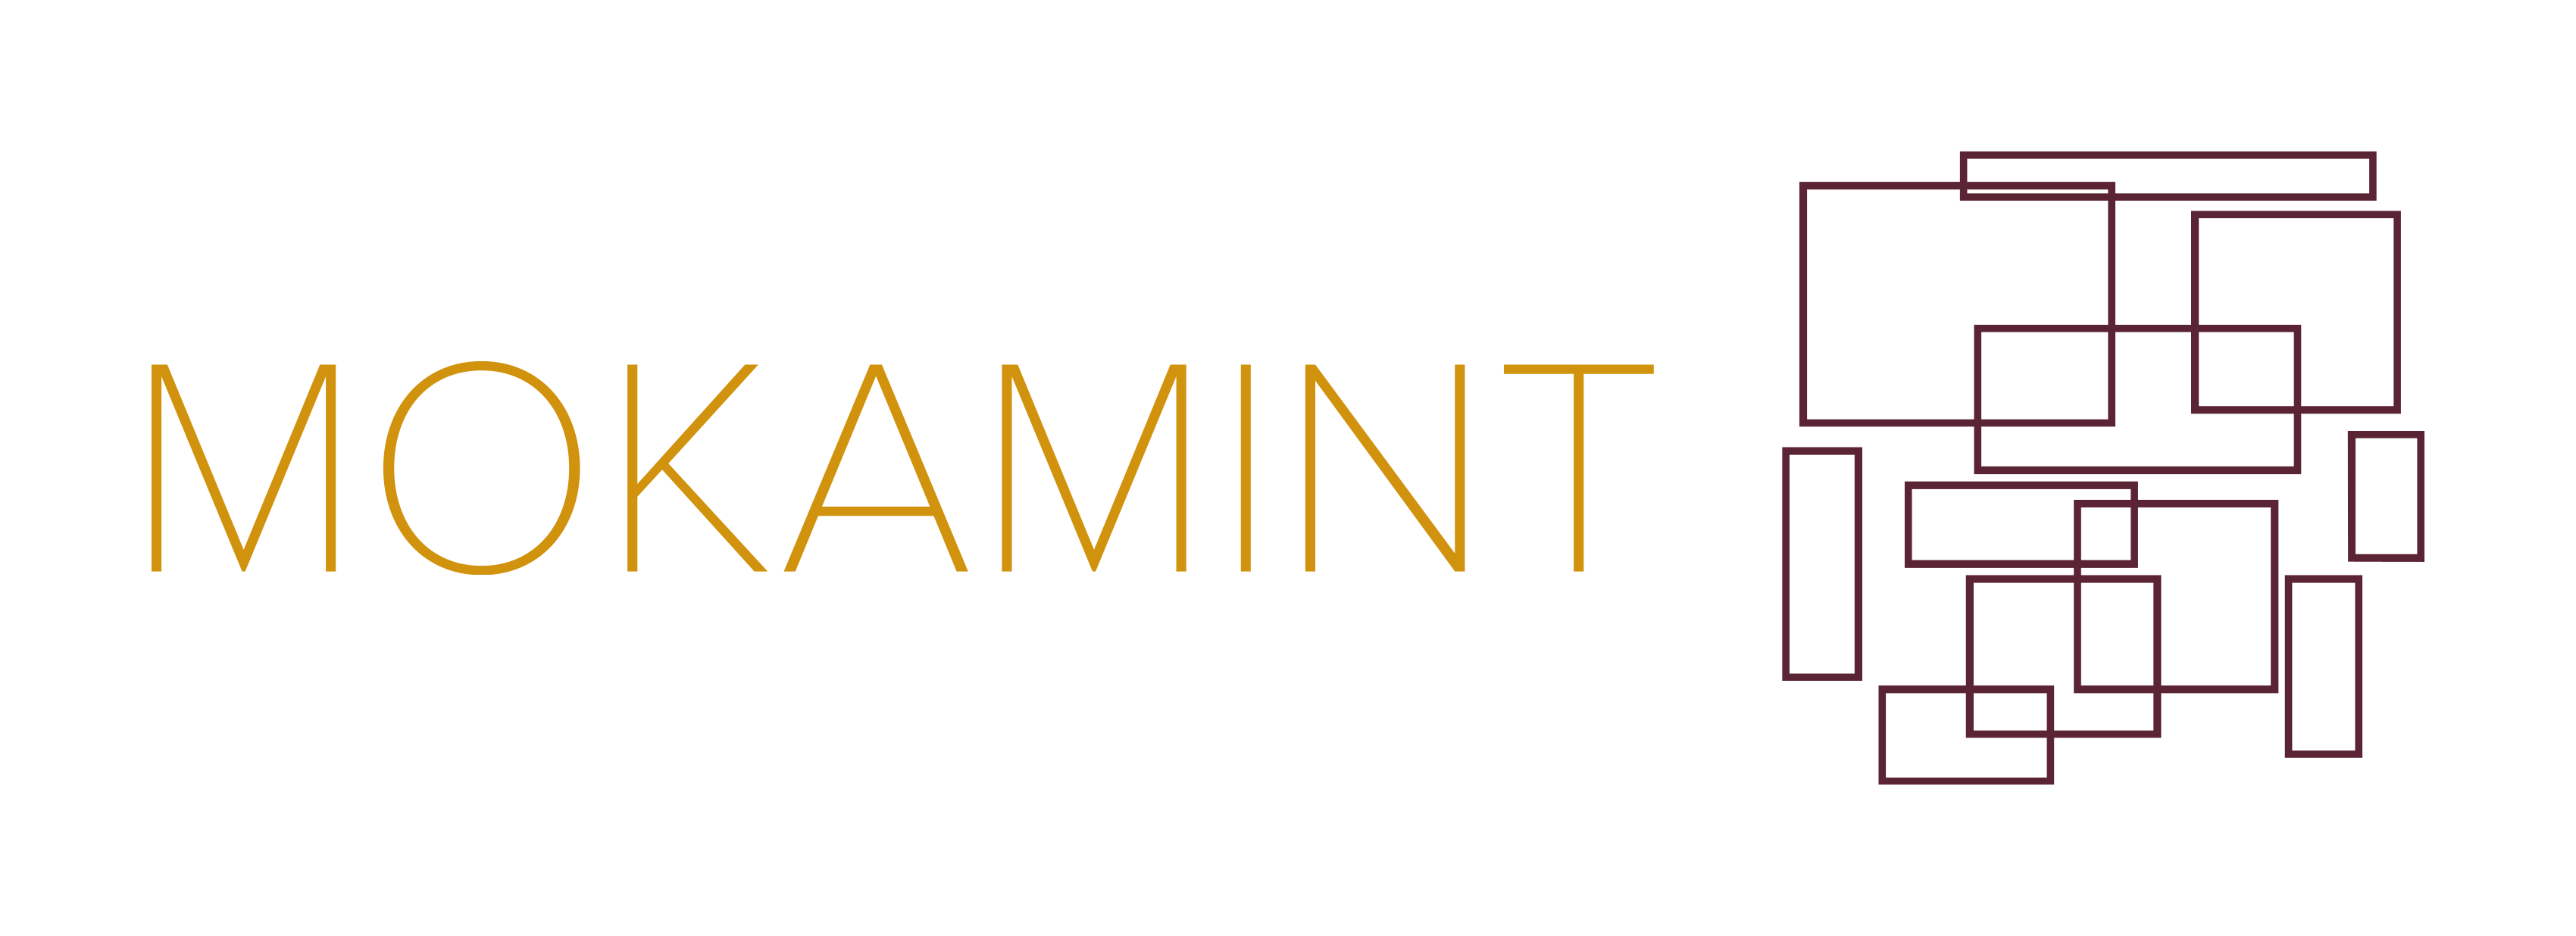
\includegraphics[width=0.4\textwidth]{pictures/mokamint_logo}\\
    \url{https://github.com/Mokamint-chain/mokamint}
  \end{center}


  \begin{center}
    A new open-source (Apache 2.0) blockchain engine
    based on proof of space, similar to Signum but \alert{generic}
    \wrt the supported \alert{application}.
  \end{center}

  \medskip

  \begin{center}
    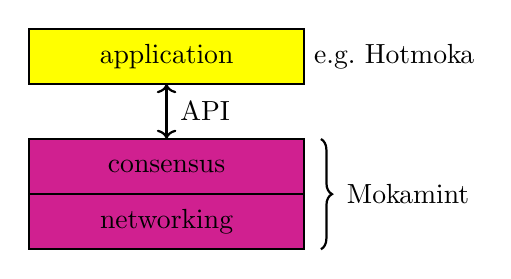
\begin{tikzpicture}[scale=0.7]
      \draw [fill=VioletRed, thick] (0,0) rectangle +(5,1);
      \draw (2.5,0.5) node{networking};
      \draw [fill=VioletRed, thick] (0,1) rectangle +(5,1);
      \draw (2.5,1.5) node{consensus};
      \draw[<->, thick] (2.5,2) -- (2.5,3);
      \draw (3.2,2.5) node{API};
      \draw [fill=Yellow, thick] (0,3) rectangle +(5,1);
      \draw (2.5,3.5) node{application};
      \draw (5,3.5) node [right] {e.g.\ Hotmoka};
      \draw [decorate,decoration={brace,amplitude=4pt},thick,xshift=0.3cm,yshift=0pt]
      (5,2) -- (5,0) node [midway,right,xshift=.2cm] {Mokamint};
    \end{tikzpicture}
  \end{center}

\end{frame}

\begin{frame}\frametitle{The Mokamint $\Leftrightarrow$ application API}

  \begin{itemize}
  \item Loosely inspired by Tendermint's Application BlockChain Interface
  \item Operational small-step semantics of an infinite state machine
  \end{itemize}

  \bigskip

  \begin{algorithm}[H] 
    \caption{Execution of the transactions of a block $\beta$}
    \begin{algorithmic}[1]
      \Require{$\finalstateid$ of $\beta$'s previous block}
      \Require{selected data $\xi=(\height,\nonce,\tau,\transactions)$ of $\beta$}
      \Ensure{$\execute(\finalstateid,\xi)$}
      \Statex
      \State {$groupId$ $\gets$ {\color{red}beginBlock}($\height$, $\finalstateid$, $\tau$)}\qquad\textbf{[git checkout]}
      \For{tx $\in$ $\transactions$}
      \State {{\color{red}checkTransaction}(tx)}
      \State {{\color{red}deliverTransaction}(tx, groupId)}\hspace*{16ex}\textbf{[git add]}
      \EndFor
      \State {$\finalstateid'$ $\gets$ {\color{red}endBlock}($\nonce$, groupId)}\hspace*{8.5ex}\textbf{[git add]}
      \State {{\color{red}commitBlock}($\finalstateid'$, groupId)}\hspace*{14.1ex}\textbf{[git commit]}
      \State \Return {$\finalstateid'$}
    \end{algorithmic}
  \end{algorithm}
  
\end{frame}

\begin{frame}{The testnet at \url{ws://panarea.hotmoka.io}}

  \begin{center}
    \begin{tikzpicture}[scale=0.95]
      \draw [fill=VioletRed,thick] (0,1) rectangle +(3,1.5);
      \draw[-, thick,dashed] (1.5,0.25) -- (1.5,1);
      \draw [fill=Yellow,thick] (0,-0.75) rectangle +(3,1);
      \draw (1.5,-0.25) node {{\scriptsize peer1 (Hotmoka)}};
      \draw (1.5,2) node {{\scriptsize peer1 (Mokamint)}};
      \draw (1.5,1.5) node {{\scriptsize 8dE4pHgtvFAXgB\ldots}};
      \draw [fill=VioletRed,thick] (0,4) rectangle +(3,1.5);
      \draw[-, thick,dashed] (1.5,5.5) -- (1.5,6.25);
      \draw [fill=Yellow,thick] (0,6.25) rectangle +(3,1);
      \draw (1.5,6.75) node {{\scriptsize peer2 (Hotmoka)}};
      \draw (1.5,5) node {{\scriptsize peer2 (Mokamint)}};

      \draw (4.3,6.75) node {\leftplug};
      \draw (4.3,6.25) node {{\scriptsize remote client}};
      \draw[-, thick] (3,6.75) -- (4,6.75);
      \draw (5.5,6.75) node {{\scriptsize port 80}};
      
      \draw (1.5,4.5) node {{\scriptsize AhYvJj737BtY24\ldots}};

      \draw [fill=lightred,thick] (4,4.85) rectangle +(4,0.8);
      \draw (5.5,5.25) node {{\scriptsize GaWKnFs1s2syow\ldots}};
      \draw (6,5.9) node {{\scriptsize local miner}};
      \draw (7.4,5.25) node {\ssd};
      \draw[-, thick] (3,5.25) -- (4,5.25);

      \draw (4.3,4.1) node {\leftplug};
      \draw (4.3,3.6) node {{\scriptsize remote miner}};
      \draw[-, thick] (3,4.1) -- (4,4.1);
      \draw (5.6,4.1) node {{\scriptsize port 8026}};

      \draw [fill=lightred,thick] (4,2) rectangle +(4,0.8);
      \draw (6,3.1) node {{\scriptsize local miner}};
      \draw (5.5,2.4) node {{\scriptsize FbXZjuFsZvQ1Ae\ldots}};
      \draw (7.4,2.4) node {\ssd};
      \draw[-, thick] (3,2.4) -- (4,2.4);

      \draw[-, thick, dashed] (1.5,2.5) -- (1.5,4);
      \draw (0.8,2.7) node {{\scriptsize port 8030}};
      \draw (0.8,3.7) node {{\scriptsize port 8032}};

      \draw (4.3,1.1) node {\leftplug};
      \draw (4.3,0.6) node {{\scriptsize remote miner}};
      \draw[-, thick] (3,1.1) -- (4,1.1);
      \visible<1>{\draw (5.6,1.1) node {{\scriptsize port 8025}};}
      
      \draw (4.3,-0.2) node {\leftplug};
      \draw (4.3,-0.7) node {{\scriptsize remote client}};
      \draw[-, thick] (3,-0.2) -- (4,-0.2);
      \draw (5.6,-0.2) node {{\scriptsize port 8001}};

      \visible<2>{
        \draw [fill=verylightgray,dashed] (6.3,0.2) rectangle +(6,1.6);
        \draw[-, thick, dashed] (4.8,1.1) -- (6.4,1.1);
        \draw (5.6,1.4) node {{\scriptsize port 8025}};
        \draw[-, thick] (7.15,1.1) -- (8.1,1.1);
        \draw [fill=lightred,thick] (8.2,0.7) rectangle +(4,0.8);
        \draw (6.8,1.1) node {\rightplug};
        \draw (10.1,0.4) node {{\scriptsize local miner in our machine}};
        \draw (9.5,1.1) node {{\scriptsize our public key}};
        \draw (11.6,1.1) node {\ssd};
      }
    \end{tikzpicture}
  \end{center}

\end{frame}

\begin{frame}[fragile]{Create your own small plot file ($5000$ nonces)}

  \begin{greenbox}{Enter the Mokamint container, run subsequent commands inside it}
\begin{verbatim}
docker run --rm -it mokamint/mokamint:1.6.1 /bin/bash
\end{verbatim}
  \end{greenbox}

  \pause
  \bigskip

  \begin{greenbox}{Create your key pair as a miner}
\begin{verbatim}
mokamint-node keys create miner.pem
\end{verbatim}
  \end{greenbox}

  \pause
  \bigskip

  \begin{greenbox}{Create a plot with your key pair as creator}
\begin{verbatim}
MINER_PUBLIC_SERVICE_URI=ws://panarea.hotmoka.io:8025
PLOT_SIZE="5000"
PUBLIC_KEY_MINER_BASE58="use the key printed above"
config-miner
\end{verbatim}
  \end{greenbox}

\end{frame}

\begin{frame}[fragile]{Become a miner of the Mokamint+Hotmoka testnet}

  \begin{greenbox}{Use the plot file that you created}
\begin{verbatim}
MINER_PUBLIC_SERVICE_URI=ws://panarea.hotmoka.io:8025 mine
\end{verbatim}
(Terminate with ENTER or leave it in background with ctrl+p, ctrl+q)
  \end{greenbox}

  \begin{center}
    You can use a minimalistic machine (250\$)\\
    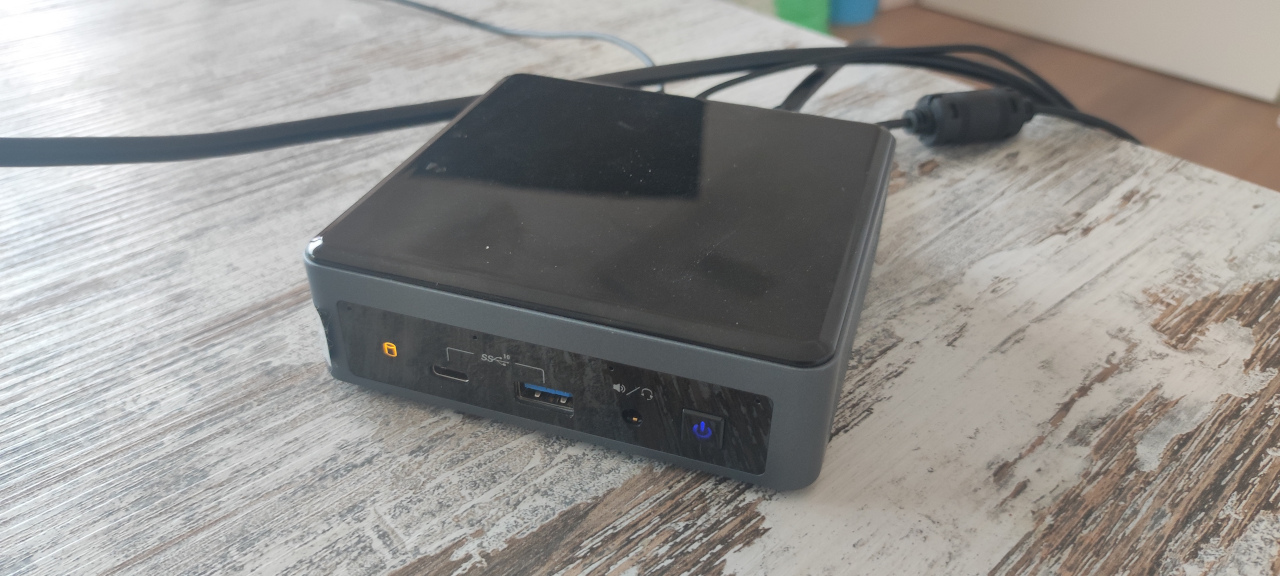
\includegraphics[width=8cm]{pictures/my_machine}
  \end{center}
  
\end{frame}

\begin{frame}[fragile]{Become a miner of the Mokamint+Hotmoka testnet}

  Since proof of space is computationally inexpensive, you can also mine
  with your $150\$$ mobile phone!

  \medskip

  \begin{greenbox}{Install the Mokaminter app from Google Play}
    \url{https://play.google.com/store/apps/details?id=io.mokamint.android.mokaminter}
  \end{greenbox}

  \begin{center}
    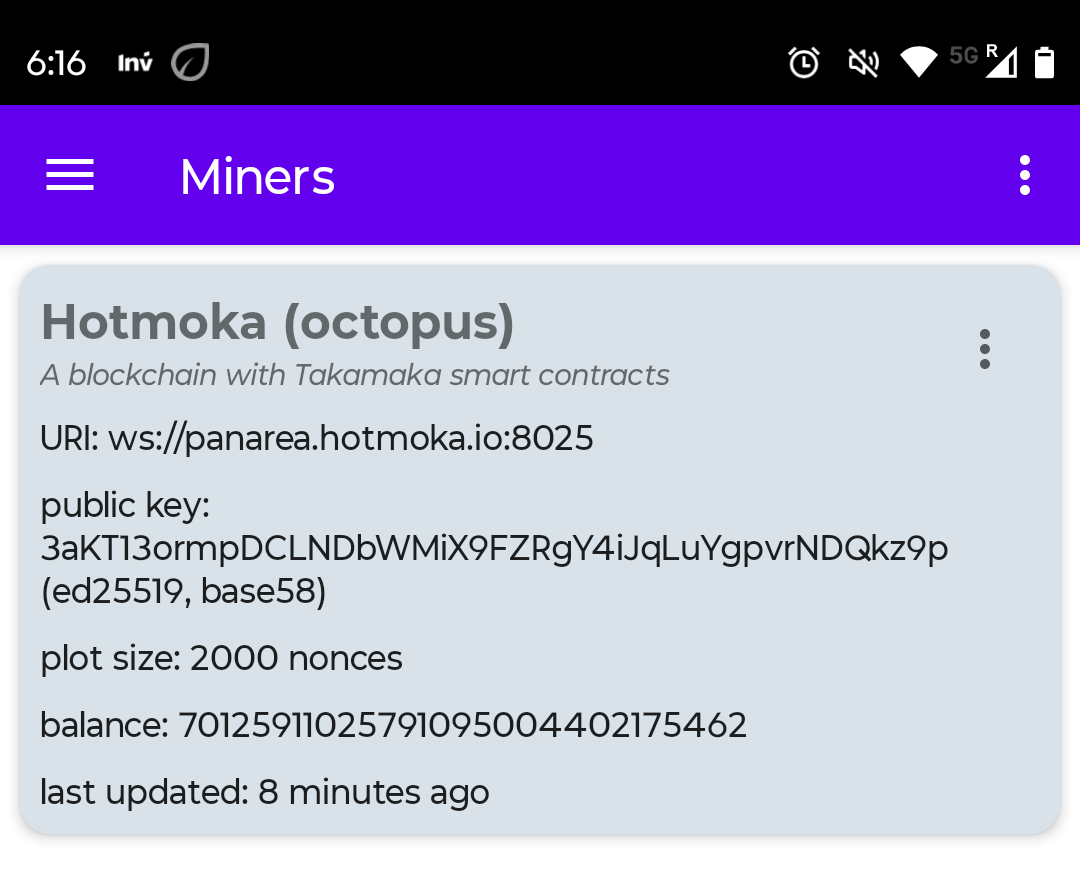
\includegraphics[width=5.5cm]{pictures/Mokaminter}
  \end{center}
  
\end{frame}

\begin{frame}[fragile]{Interact with the Mokamint node}

  \begin{greenbox}{Show the topmost $20$ block hashes of the chain and look for your key}
\begin{verbatim}
mokamint-node chain ls 20 --uri ws://panarea.hotmoka.io:8030
  | grep you key
\end{verbatim}
  \end{greenbox}

  \bigskip\pause
  \begin{greenbox}{Show the topmost block of the blockchain}
\begin{verbatim}
  mokamint-node chain show head --full
    --uri ws://panarea.hotmoka.io:8030
\end{verbatim}
  \end{greenbox}

  \bigskip\pause
  \begin{greenbox}{List the miners connected to the node}
\begin{verbatim}
mokamint-node miners ls --uri ws://panarea.hotmoka.io:8030
\end{verbatim}
  \end{greenbox}

\bigskip
  Exit the container at the end.
  
\end{frame}

\section{Experiments with Hotmoka}

\begin{frame}
  \frametitle{Hotmoka}

  \begin{center}
    
\includegraphics[width=5cm]{pictures/hotmoka_logo}
  \end{center}

  \begin{greenbox}{\url{https://github.com/Hotmoka/hotmoka}}
    An application for Mokamint whose transactions are OO-based:
    \begin{itemize}
    \item code installations
    \item object creation
    \item method calls on objects
    \item methods are implemented in Takamaka (subset of Java)
    \item the blockchain stores the compiled Java bytecode only
    \item see full online tutorial at the above Github page
    \end{itemize}
  \end{greenbox}

\end{frame}

\begin{frame}\frametitle{An OO state (hash is sha256)}

  \begin{center}
    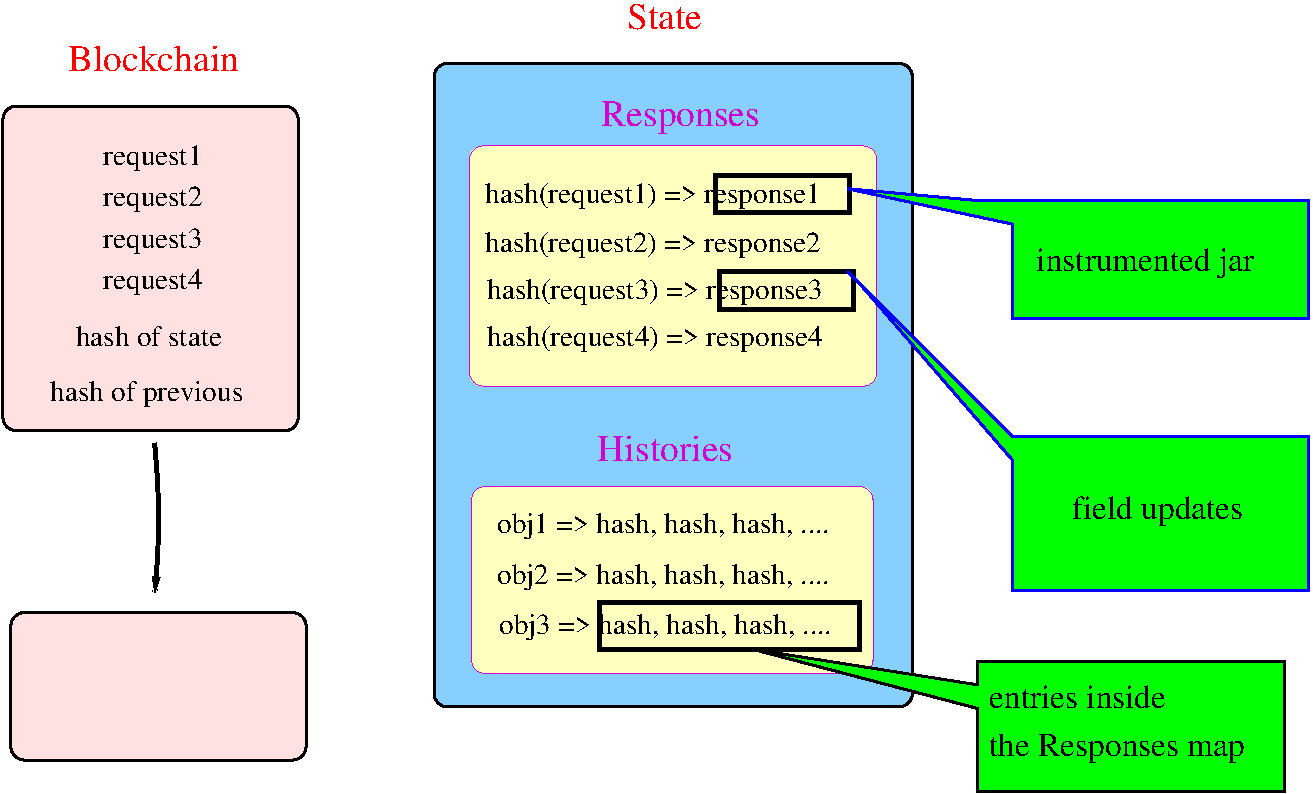
\includegraphics[width=\textwidth,clip=false]{pictures/hotmoka-structure.pdf}
  \end{center}

\end{frame}

\begin{frame}[fragile]\frametitle{Creation of an account}

  We need an account to play, already charged with some cryptocurrency:

  \begin{itemize}
  \item collect cryptocurrency by mining
  \item ask cryptocurrency to a friend
  \item use the faucet of the testnet
  \item buy cryptocurrency at an exchange (not possible for Hotmoka yet)
  \end{itemize}

  Let's go for the faucet...

\end{frame}

\begin{frame}[fragile]\frametitle{Creation of two accounts (repeat twice)}

  \begin{greenbox}{Create a key pair}
{\small\begin{verbatim}
moka keys create --name fausto.pem
\end{verbatim}}
  \end{greenbox}

  \pause
  \bigskip
  \begin{greenbox}{Create an account with that public key}
{\small\begin{semiverbatim}
moka accounts create faucet 100000000000000
  your-key-here --uri ws://panarea.hotmoka.io:8001

{\color{red}A new account {\color{blue}c3ca5522...#0} has been created.}
\end{semiverbatim}}
(That URI is the default, so we won't add it anymore)
  \end{greenbox}

  \pause
  \bigskip
  \begin{greenbox}{Rename the key pair with the address of the account object}
{\small\begin{verbatim}
mv fausto.pem address-printed-above.pem
\end{verbatim}}
  \end{greenbox}

  \pause\bigskip
  \begin{greenbox}{An actual Java object!}
{\small\begin{semiverbatim}
  moka objects show {\color{blue}c3ca5522...#0} --api
\end{semiverbatim}}
  \end{greenbox}

\end{frame}

\begin{frame}\frametitle{The Takamaka programming language}

  Takamaka is a small, deterministic subset of Java. It uses code annotations to implement contract-based aspects:

  \begin{itemize}
  \item {\color{blue}\<@FromContract>} annotates something that can only be called by a contract,
    not by any other code; hence, it has a {\color{blue}\<caller()>}
  \item {\color{blue}\<@Payable>} annotates something whose execution requires to pay some
    cryptocurrency units
  \item {\color{blue}\<@View>} annotates something whose execution can be run for free,
    without paying for its gas: it must not generate any update at its end
    (\emph{pure} code)
  \end{itemize}

  \bigskip
  Takamaka comes equipped with a {\color{blue}support library}
  (\<io-takamaka-code>) that defines such annotations and
  other typical classes that are useful
  for programming smart contracts.

\end{frame}

\begin{frame}[fragile]\frametitle{Let us install our jar in blockchain}

  \begin{greenbox}{We let Fausto pay}
{\small\begin{semiverbatim}
  moka jars install {\color{blue}c3ca5522...#0} io-hotmoka-experiments-1.0.jar
  {\color{red}The jar has been installed at {\color{blue}c710a9083787...}}
\end{semiverbatim}}

  Note: the presence of the key pair \texttt{c3ca5522...\#0.pem} in
  our directory authorizes us to charge that operation on our account.
  \end{greenbox}

\end{frame}

\begin{frame}\frametitle{Installation of a jar in blockchain}

  Each jar that gets installed in a Hotmoka node undergoes two processes:

  \begin{enumerate}
  \item Verification: absence of frequent errors
    \begin{itemize}
    \item non-deterministic or non-terminating library code is not used
    \item no synchronization
    \item no native code
    \item no \emph{dangerous} bytecodes
    \item no finalizers
    \item no static fields (mostly)
    \item code annotations are used correctly
    \item \ldots
    \end{itemize}
  \item Instrumentation
    \begin{itemize}
    \item fields of \<Storage> classes get duplicated to spot updates
    \item gas metering is weaved into the code
    \item code annotations get enforced \emph{by magic}
    \item \ldots
    \end{itemize}
  \end{enumerate}

\end{frame}

\begin{frame}[fragile]\frametitle{Let us create an instance of \texttt{SimplePonzi} in blockchain}

  \begin{greenbox}{We let Fausto pay}
{\small\begin{semiverbatim}
  moka objects create {\color{blue}c3ca5522...}
    io.hotmoka.experiments.SimplePonzi
    --classpath {\color{blue}c710a9083787...}

  {\color{red}A new object {\color{blue}d2976345539...#0} has been created}
\end{semiverbatim}}
  \end{greenbox}

  \pause
  \bigskip
  \begin{greenbox}{Check the state of the object}
{\small\begin{semiverbatim}
moka objects show {\color{blue}d2976345539...#0}
\end{semiverbatim}}
  \end{greenbox}

\end{frame}

\begin{frame}[fragile]\frametitle{Call the \texttt{invest} method of the object}

  \begin{greenbox}{We let Fausto invest}
{\small\begin{semiverbatim}
  moka objects call {\color{blue}c3ca5522...}
    io.hotmoka.experiments.SimplePonzi invest 1000
    --receiver {\color{blue}d2976345539...#0}
  moka accounts show {\color{blue}c3ca5522...}
\end{semiverbatim}}
  \end{greenbox}

  \pause
  \bigskip

  \begin{greenbox}{We then let Alice invest and check that Fausto receives 2000}
{\small\begin{semiverbatim}
  moka objects call {\color{blue}79a2e177...}
    io.hotmoka.experiments.SimplePonzi invest 2000
    --receiver {\color{blue}d2976345539...#0}
  moka accounts show {\color{blue}c3ca5522...}
\end{semiverbatim}}
  \end{greenbox}

\end{frame}

\begin{frame}[fragile]\frametitle{Call the \texttt{invest} method of the object and fail}

  \begin{greenbox}{We let Fausto invest}
{\small\begin{semiverbatim}
  moka objects call {\color{blue}c3ca5522...}
    io.hotmoka.experiments.SimplePonzi invest 2200
    --receiver {\color{blue}d2976345539...#0}

  {\color{red}The transaction failed with message:
  you must invest more than 2200@SimplePonzi.java:50}

Gas consumption:
 * total: 1000000
   * for CPU: 16187
   * for RAM: 8503
   * for storage: 18800
   * {\color{red}for penalty: 956510}
\end{semiverbatim}}
  \end{greenbox}

\end{frame}

\begin{frame}[fragile]\frametitle{Check the current investment before investing}

  \begin{greenbox}{This is very cheap\ldots}
{\small\begin{semiverbatim}
  moka objects call {\color{blue}c3ca5522...}
    io.hotmoka.experiments.SimplePonzi getCurrentInvestment
    --receiver {\color{blue}d2976345539...#0}

{\color{red}The method returned:
2000}

(no gas has been consumed)
\end{semiverbatim}}
  \end{greenbox}

\end{frame}

\begin{frame}\frametitle{The execution of a method (or constructor)}

  \begin{greenbox}{The request specifies}
    \begin{itemize}
    \item payer object, receiver object and actual arguments (\emph{input})
    \item classpath, signature of the method
    \item nonce, chain id, gas price, gas limit
    \item signature of the request
    \end{itemize}
  \end{greenbox}

  \bigskip

  \begin{greenbox}{The computation of the response (ie, the execution of the request)}
    \begin{enumerate}
    \item create a classloader from some jars in blockchain
    \item reconstruct, from the state, RAM objects for \emph{input}
    \item execute the method on a normal Java Virtual Machine (in RAM)
    \item at the end, identify updates to fields of objects reachable from \emph{input}
      or return value
    \item pack those updates into a response (RAM objects destroyed now)
    \item put request/response in state, expanding histories
    \end{enumerate}
  \end{greenbox}

\end{frame}

\begin{frame}[fragile]\frametitle{How can Hotmoka identify updates to fields of objects?}

  \begin{greenbox}{The original code}
    \begin{semiverbatim}
      public class C \{
        public {\color{blue}int i;}
        public void foo() \{
          {\color{blue}i} = 42;
        \}
      \}
    \end{semiverbatim}
  \end{greenbox}

  \begin{center}
    No way to know if \<i> changed its value during the execution of \<foo()>
  \end{center}

\end{frame}

\begin{frame}[fragile]\frametitle{How can Hotmoka identify updates to fields of objects?}

  \begin{greenbox}{The instrumented code}
    \begin{semiverbatim}
      public class C {\color{red}extends Storage} \{
        public {\color{blue}int i, old\_i;} // aliased at method start
        public void foo() \{
          {\color{blue}i} = 42;
        \}
      \}
    \end{semiverbatim}
  \end{greenbox}

  \begin{center}
    \<i> changed its value during the execution of \<foo()> iff at the end \<i>$\not=$\<old\_i>
  \end{center}

\end{frame}

\begin{frame}[fragile]\frametitle{How can Hotmoka enforce gas limits?}

  \begin{greenbox}{The original code}
    \begin{semiverbatim}
      public class C \{
        public void foo() \{
          while (...) \{
            ...
          \}
        \}
      \}
    \end{semiverbatim}
  \end{greenbox}

  \begin{center}
    This loop might run for very long or even forever
  \end{center}

\end{frame}

\begin{frame}[fragile]\frametitle{How can Hotmoka enforce gas limits?}

  \begin{greenbox}{The instrumented code}
    \begin{semiverbatim}
      {\color{blue}static long counter;}
      public class C \{
        public void foo() \{
          while (...) \{
            {\color{blue}if (counter++ >= gaslimit)
              throw new OutOfGasError();}
            ...
          \}
        \}
      \}
    \end{semiverbatim}
  \end{greenbox}

  \begin{center}
    Actual gas costs are more fine-grained
  \end{center}

\end{frame}

% fausto: 79a2e1776da0763aee972f8012af170e21a61e4d7d6da3b340cc990527f02f9e#0
% alice: c3ca5522d5ea850c9dcb9dc1a204780d08826f8acda28814da59685705ea7676#0
% jar: c710a9083787b683df47ffd04e1e1033ff0ac61c01d5ad617fb7a939be8efae4
% simple ponzi: d2976345539a19abc40e7c357d701641931f1444b543e53a72014165ac3783d5#0

\end{document}
